\documentclass[11pt,a4paper]{article}
\usepackage[margin=2.6cm]{geometry}
\usepackage{amsmath,amssymb,amsthm,mathtools}
\DeclareTextSymbol{\textsection}{OMS}{120}
\DeclareTextSymbolDefault{\textsection}{OMS}
\DeclareTextSymbol{\textdagger}{OMS}{121}
\DeclareTextSymbolDefault{\textdagger}{OMS}
\DeclareTextSymbol{\textdaggerdbl}{OMS}{122}
\DeclareTextSymbolDefault{\textdaggerdbl}{OMS}
\DeclareTextSymbol{\textasteriskcentered}{OMS}{3}
\DeclareTextSymbolDefault{\textasteriskcentered}{OMS}
\DeclareTextSymbol{\textbullet}{OMS}{15}
\DeclareTextSymbolDefault{\textbullet}{OMS}
\usepackage{booktabs,longtable,array}
\usepackage{graphicx}
\usepackage{xcolor}
\usepackage{tikz}
\usetikzlibrary{calc}
\usepackage{enumitem}
\usepackage[font=small,labelfont=bf]{caption}
\usepackage[expansion=false]{microtype}
\usepackage[colorlinks=true,linkcolor=black,citecolor=black,urlcolor=black]{hyperref}

\newtheorem{theorem}{Theorem}[section]
\newtheorem{proposition}[theorem]{Proposition}
\newtheorem{lemma}[theorem]{Lemma}
\newtheorem{corollary}[theorem]{Corollary}
\theoremstyle{definition}
\newtheorem{definition}[theorem]{Definition}
\theoremstyle{remark}
\newtheorem{remark}[theorem]{Remark}

\newtheorem*{theoremA}{Theorem A}
\newtheorem*{theoremB}{Theorem B}

% draft markers: everything in red is to be completed before submission
\newcommand{\pending}[1]{{\color{red!75!black}[#1]}}

\newcommand{\Sri}{\'Sr\={\i}}
\newcommand{\br}[2]{[#1\,#2]}
\newcommand{\yy}[2]{y_{#1#2}}
\newcommand{\Mo}{\mathcal{M}}
\newcommand{\V}{\mathcal{V}}
\newcommand{\Lam}{\mathcal{L}}
\newcommand{\softplus}{\operatorname{sp}}
\newcommand{\Tstar}{T^{*}}

\title{Extended circular-arc \Sri{} Yantras}
\author{Claude (Anthropic)\thanks{Claude Opus 5.5, model string \texttt{claude-opus-5-5}, run as an agent
with file, shell and browser access. Work carried out in September and October 2026.}
\and Michael Kopp\thanks{Corresponding author: \texttt{mkopp911@gmail.com}}}
\date{October 2026}

\renewcommand{\topfraction}{0.92}
\renewcommand{\textfraction}{0.06}
\renewcommand{\floatpagefraction}{0.8}
\begin{document}
\maketitle

\begin{abstract}
\noindent
Carrying the outermost side of the \Sri{} Yantra on each hand out until it closes into a triangle of
its own gives a figure of eleven triangles, six pointing down and five up. The two new triangles have as
legs the curve through the three outer corners of the opposite family, and between them and the
circumscribed circle they cut a further ring of cells. We prove two results about these extended
\Sri{} Yantras. First, none has straight sides: no laminar straight \Sri{} Yantra has the outer corners of
both families collinear with a laminar extension. A projective symmetry of the straight figure reduces
the statement to one about thirteen points on the projective line, eight equations and twenty-five
inequalities between products of cross-ratios, and this statement is decided by a computer-assisted
proof. The configuration space is covered by $58{,}786$ cones, one for each triangulation of a
$13$-gon, on each of which every condition is a linear form in logarithmic coordinates plus corrections
that vanish exponentially towards the vertex of the cone. Each cone is closed by interval arithmetic and
by linear-programming certificates verified in exact rational arithmetic, except near one vertex of the
associahedron, where the equations and the inequalities approach one another and an asymptotic analysis
in adapted coordinates decides. Second, with circular arcs the extension exists: we give two laminar
figures, whose new rings have ten and fourteen cells, by straightedge and compass constructions in which
every incidence holds by construction, with $22$ and $20$ free parameters.
\end{abstract}

\section{Introduction}

The \Sri{} Yantra is the union of nine triangles, five pointing down and four up, symmetric about a
common axis, whose sides are required to pass through a large number of common points. Chiodo
\cite{Chiodo} gave a straightedge and compass construction of the straight figure and identified its
essential step as a circle--line--point problem of Apollonius. In \cite{CK} the twenty-seven sides were
replaced by circular arcs, every classical incidence was kept, and the fourteen outer corners of the
figure were placed on the circumscribed circle; the result is an $18$-dimensional family reached by a
straightedge and compass construction in which every coincidence holds identically. We follow the
notation of \cite{Chiodo,CK} throughout.

The traditional diagram continues outwards. Around the nine triangles lie the enclosures of eight and
sixteen lotus petals, three circles and the square \emph{bh\=upura}; inside the triangles the
outermost enclosure is the \emph{caturda\'s\=ara}, the ring of fourteen triangles whose outer vertices are
the fourteen outer corners. The present paper concerns the natural question of whether the triangular
structure itself can be continued by one more ring.

The rings of the classical figure are nested in a way that indicates how such a ring is to be added
(Figure~\ref{fig:kites}). For an upward triangle $U$ and a downward triangle $D$ whose apex lies below
that of $U$, we call the quadrilateral bounded by their legs, from the two apexes to the two points where
a leg of $U$ crosses a leg of $D$, the \emph{kite} of $U$ and $D$. The central triangle lies in the kite of
$U_3$ and $D_5$, with its two base corners on the legs of $U_3$. Each of the rings of eight, ten and ten
triangles around it has its top and bottom vertices at the apexes of one kite and its other outer
vertices on the legs of the next, the kites being, from the inside, those of $U_3$ and $D_5$, $U_4$ and
$D_4$, $U_2$ and $D_2$, and $U_1$ and $D_1$; the ring of fourteen has its top and bottom vertices at the
apexes of the last. On each side of the axis these are twelve incidences of a vertex with a leg, and they
are exactly Chiodo's twelve concurrences (Section~\ref{sec:straight}). Read from the centre outward, the
figure is built ring by ring: the lines already drawn are carried on beyond their kite, they cut out the
next ring, and the outer vertices of that ring fix the next kite.

\begin{figure}[t]
\centering
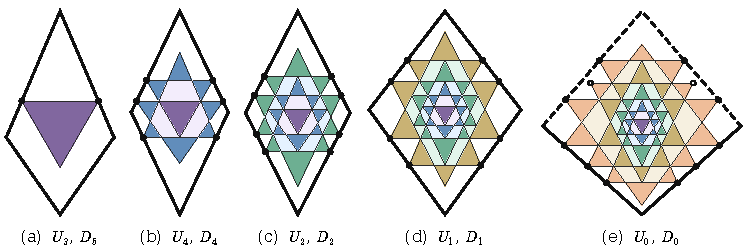
\includegraphics[width=\textwidth]{../figs/kites.pdf}
\caption{A laminar straight \Sri{} Yantra of classical type in which the outer corners of $U_1$, $U_2$, $U_3$
are collinear, built from the centre outward.
(a)~The central triangle, with its base corners (dots) on the legs of $U_3$, in the kite of $U_3$ and
$D_5$. (b)--(d)~The rings of eight, ten and ten triangles, each with its top and bottom vertices at the
apexes of the previous kite and its other outer vertices (dots) on the legs of the next: the kites of
$U_4$ and $D_4$, of $U_2$ and $D_2$, and of $U_1$ and $D_1$. (e)~The ring of fourteen. Its outer vertices
off the axis are the outer corners of $D_1$, $D_2$, $D_3$ and of $U_1$, $U_2$, $U_3$, and a kite through
them is the extension. Here the corners of $U_1$, $U_2$, $U_3$ lie on the lower legs of the kite (solid);
the upper legs, drawn through the corners of $D_1$ and $D_3$ (dashed), miss the corner of $D_2$ (open
dots). Each ring is shaded in its own tone, lighter outward, and the cells between consecutive rings in a
pale tint of the inner one. Each panel is scaled to its kite.}
\label{fig:kites}
\end{figure}

In this reading the ring of fourteen is the last ring built, and a further ring needs a fifth kite,
whose legs carry the outer corners of the ring of fourteen. In the traditional drawing the outer corners
of the three largest downward triangles lie close to a common line, and so do those of the three largest
upward triangles; in the yantra of Figure~\ref{fig:kites} the upward triple is collinear and the
downward triple is not. If each triple lies exactly on a common side, that side and its mirror image close
into a new triangle: an upward triangle $U_0$ whose legs pass through the outer corners of $D_1$, $D_2$,
$D_3$, and a downward triangle $D_0$ whose legs pass through those of $U_1$, $U_2$, $U_3$. Their kite is
the fifth kite, and the figure has eleven triangles, six down and five up. Carried on beyond the fifth
kite, as at every earlier step, the sides of $U_0$ and $D_0$ cut out a new ring. With straight sides it
consists of the tips of $U_0$ and $D_0$ at their apexes and the four triangles at the corners of their
bases (Figure~\ref{fig:nearmiss}), the six cells of the pattern without walls in Section~\ref{sec:arcs};
with the circular arcs of Part~II it is cut out of the disc between the
yantra and the circumscribed circle, the rim. We
call such a figure an \emph{extended} \Sri{} Yantra.

The figure is asked to keep the character of the original in one respect that is not an incidence.
Within each family the triangles of the \Sri{} Yantra do not cross: no leg of a downward triangle meets
the leg of another downward triangle, and likewise upwards. We call this property \emph{laminarity}
(Definition~\ref{def:laminar}); it is what gives the figure its characteristic layered appearance, and it
is the property any extension has to preserve.

\subsection*{What is proved}

\begin{theoremA}
There is no straight extended \Sri{} Yantra of classical type. That is, in no straight \Sri{} Yantra whose
nine triangles are laminar can the outer corners of $D_1$, $D_2$, $D_3$ and those of $U_1$, $U_2$, $U_3$
both be collinear in such a way that the two triangles they span contain their families and the eleven
triangles are laminar.
\end{theoremA}

Figure~\ref{fig:nearmiss} shows how close the straight figure comes. Its eleven triangles are laminar
and both triples of outer corners are collinear, so that the fifth kite exists, and every incidence of
the \Sri{} Yantra holds except one: the corner of $U_4$, an outer vertex of the inner ring of ten, misses
the leg of $D_2$, a side of the third kite. Such figures form a family of dimension four, and Theorem~A
says that along it the miss cannot be brought to zero without breaking laminarity. The two are in
tension well before that point. Laminarity is a finite list of inequalities (Section~\ref{sec:straight}),
and we measure each by the ratio of its two sides minus one. In our computations the smallest of these
relative clearances can be raised to about $16\%$ when the miss is $10\%$ of the half-width of $U_4$,
and only to about $4\%$ when the miss is $4\%$; the clearances that limit it are those between the leg of
$D_4$ and the corner of $D_5$ and between the corner of $U_1$ and the side of $U_0$. The figure shown
trades closeness for legibility: its miss is $15\%$ and its smallest clearance about $20\%$.

\begin{figure}[tp]
\centering
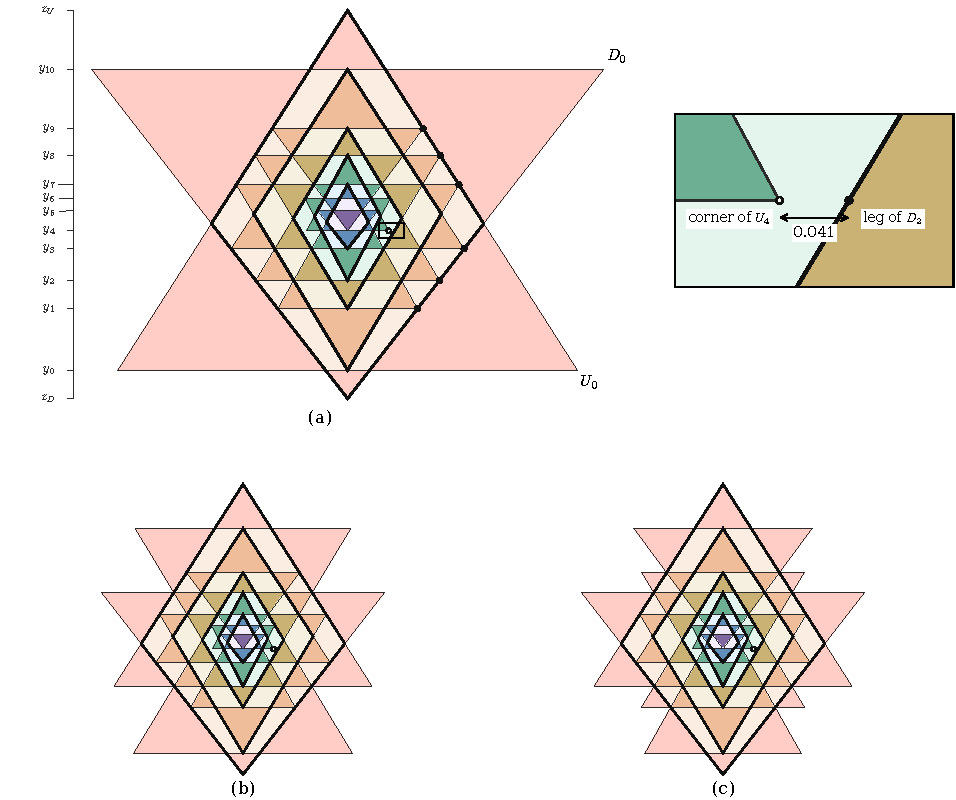
\includegraphics[width=\textwidth]{../figs/straight_nearmiss.pdf}
\caption{A laminar straight \Sri{} Yantra with both triples of outer corners collinear (dots), extended
by $U_0$ and $D_0$, shaded as in Figure~\ref{fig:kites} and with its five kites drawn heavy. (a)~The
figure as constructed. Its new ring consists of the tips of $U_0$ and $D_0$ at their apexes and the four
triangles at the corners of their bases, the six cells of the wall pattern $00$ of
Section~\ref{sec:arcs}. Of the twelve concurrences of the \Sri{} Yantra eleven hold. The twelfth, ((iii);
$t_2,t_6,t_6$) in Chiodo's notation, asks the leg of $D_2$, a side of the kite of $U_2$ and $D_2$, to pass
through the base corner of $U_4$ (open dot), and misses it by $15\%$ of the half-width of $U_4$ (right,
enlarged from the box; the number marked is the miss in units in which the yantra has height $2$).
Within the family of such figures this one was chosen for even rings and wide clearances: in each of the
rings of eight, ten, ten and fourteen triangles, and among the fourteen cells between the yantra and the
fifth kite, the largest has at most $5.5$ times the area of the smallest, and every laminarity inequality
holds with a relative margin of about $20\%$ or more. The apexes of $U_0$ and $D_0$ have been placed at
$z_U - y_{10} = y_{10} - y_9$ and $y_0 - z_D = y_2 - y_1$. The horizontal scale is free and has been
chosen for legibility; the levels $y_0, \dots, y_{10}$ and the apexes $z_D$, $z_U$ of $D_0$ and $U_0$ are
marked on the left. (b),~(c)~The same figure with triangles carried out beyond the fifth kite as in
Section~\ref{sec:arcs}, with horizontal bases in place of the arcs, in the positions of the wall patterns
$22$ and $36$ of Figure~\ref{fig:two}: the middle corner on each hand (b) and the two outermost (c). On
the straight figure these are the corners of $D_2$ and $U_2$, and of $D_3$, $D_2$ and $U_3$, $U_2$, since
the straight and the circular-arc figures order their downward bases differently
(Section~\ref{sec:figure}). The new rings have ten and fourteen cells.}
\label{fig:nearmiss}
\end{figure}

The proof has two parts of different character. The first is an exact reduction (Sections
\ref{sec:straight}--\ref{sec:thirteen}). A straight \Sri{} Yantra is determined, up to the horizontal
scale, by the eleven heights on the axis at which its apexes and bases lie, subject to four quartic
equations; its extension adds two collinearities and the apexes $z_D$, $z_U$ of the new triangles. Every
one of these conditions, and every laminarity condition, is an identity or an inequality between
products of differences of the thirteen heights in which each height occurs as often in the numerator as
in the denominator. Such products are invariant under all projective transformations of the axis, and
the problem therefore lives on the space $\Mo$ of thirteen cyclically ordered points on the projective
line modulo $\mathrm{PGL}_2(\mathbb{R})$, which has dimension ten. In $\Mo$ the eight equations cut out
a surface $\V$ and the inequalities a closed set $\Lam$, and Theorem~A follows from
\[
  \V \cap \Lam = \varnothing \qquad\text{(Theorem~\ref{thm:main}).}
\]

The second part proves this statement, and it is computer-assisted (Sections
\ref{sec:cones}--\ref{sec:certificate}). Its organising fact is that $\Mo$ is the interior of an
associahedron, and that near each of its $58{,}786$ vertices, which correspond to the triangulations of a
$13$-gon, there are coordinates in which the logarithm of every distance between two of the thirteen points
is a linear form plus a correction that vanishes exponentially fast towards the vertex. We use the logarithms of the
gaps between consecutive points; the vertices then correspond to the Cartesian trees of the gap sequence,
and each cone is a product of half-lines. On each cone the eight equations and the twenty-five
inequalities become linear conditions perturbed by small, explicitly bounded, corrections, which makes a
branch and bound over half-infinite boxes possible: a box is closed when interval arithmetic, or a linear
program whose infeasibility is certified by Farkas multipliers checked in exact rational arithmetic, shows
that it contains no point of $\V \cap \Lam$. This closes every cone except near one vertex $\Tstar$. There
$\V$ and $\Lam$ approach each other: the laminar points that satisfy seven of the eight equations
accumulate at $\Tstar$, and the residual of the eighth tends to zero with them. Near $\Tstar$ we use
coordinates adapted to the vertex, in which a combination $\Phi$ of the equations has the explicit
leading term $t_3t_4 + t_5t_6 + t_9t_{10}$ (Proposition~\ref{prop:phi}), and a certificate in those
coordinates closes the neighbourhood (Section~\ref{sec:tstar}).

With circular arcs the extension exists. The ring of cells that $U_0$ and $D_0$ cut out has, on each of its
two sites, room for up to four triangles, separated by three walls; a wall stands when the triangle behind
it is carried out to the rim, and there are $2^3 \times 2^3 = 64$ patterns of walls
(Section~\ref{sec:walls}). For two of them, with ten and fourteen cells in the new ring, we give
constructions of the kind \cite{CK} gives for the nine-triangle figure.

\begin{theoremB}
The circular-arc extended \Sri{} Yantras with the wall patterns $\{D_3\}\times\{U_2\}$ and
$\{D_1,D_3\}\times\{U_2,U_3\}$ are reached by straightedge and compass constructions from $13$ placed
corners, which carry $22$ and $20$ free real parameters, and the two poles of the rim:
\begin{enumerate}[label=(\roman*),leftmargin=2.5em]
\item after the placements the constructions take $52$ and $54$ steps, each of which is a circle through two
or three points or the meeting of a circle with a circle, the axis or the rim;
\item every incidence of the figure, including every outer node of its new ring lying on the rim, holds by
construction, each realised by exactly one step;
\item at the corners of Table~\ref{tab:seeds} the eleven triangles are laminar.
\end{enumerate}
\end{theoremB}

Figure~\ref{fig:two} shows the two figures of Theorem~B. Section~\ref{sec:constructions} gives the
constructions; the accompanying viewer draws both and the GeoGebra files carry them as command lists.

\begin{figure}[tp]
\centering
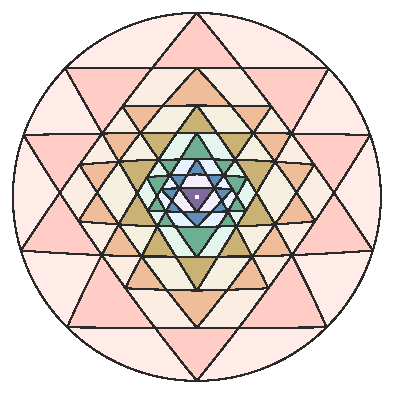
\includegraphics[width=0.46\textwidth]{../figs/arcx2.pdf}\hfill
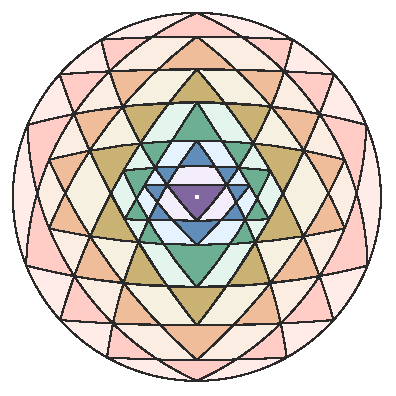
\includegraphics[width=0.46\textwidth]{../figs/arcx3.pdf}
\caption{The two constructed extended \Sri{} Yantras of Theorem~B, with ten (left) and fourteen (right)
cells in the ring between the yantra and the rim, shaded as in Figure~\ref{fig:kites}; the ground between
the new ring and the rim takes the pale tint of the new ring. Every node and every arc is produced by
straightedge and compass from the placed corners; the outer nodes of the ring are on the rim by
construction. Figure~\ref{fig:nearmiss}(b),~(c) shows the straight figure carried out in the same
positions.}
\label{fig:two}
\end{figure}

\paragraph{Organisation.}
Section~\ref{sec:figure} fixes the objects. Part~I (Sections
\ref{sec:straight}--\ref{sec:certificate}) proves Theorem~A. Part~II (Sections
\ref{sec:arcs}--\ref{sec:constructions}) treats the circular-arc figures and proves Theorem~B.
Section~\ref{sec:software} describes the software and the data that accompany the paper.

%======================================================================
\section{The extended figure}\label{sec:figure}

\subsection{Notation}
We use the labels of the accompanying software: $D_1,\dots,D_5$ for the downward and $U_1,\dots,U_4$ for
the upward triangles. Each triangle is isosceles with its apex on the axis $x = 0$ and its base
perpendicular to the axis, or, for arcs, symmetric about it; its two remaining sides are its \emph{legs}.
The base corner on the right is the triangle's \emph{corner}. Chiodo's numbering $t_1, \dots, t_9$ orders
the triangles by the height of their bases from the top and therefore depends on the figure; on the
straight figures considered in Part~I it reads
\[
  t_1 = D_3,\; t_2 = D_2,\; t_3 = D_1,\; t_4 = D_4,\; t_5 = D_5,\; t_6 = U_4,\; t_7 = U_1,\; t_8 = U_2,\;
  t_9 = U_3,
\]
and on the circular-arc figures of Part~II the first three are instead $t_1 = D_1$, $t_2 = D_3$,
$t_3 = D_2$ \cite{CK}. Chiodo's conditions are recalled in Section~\ref{sec:straight}. The upward
triangles form one \emph{family} and the downward triangles the other; the new triangles $U_0$ and $D_0$
belong to the upward and the downward family respectively.

\subsection{Laminarity}

\begin{definition}\label{def:laminar}
A figure of triangles divided into two families is \emph{laminar} if no leg of a triangle meets a leg of
another triangle of the same family.
\end{definition}

The incidences of the \Sri{} Yantra never ask two legs of one family to meet: each of Chiodo's triple
points lies on one downward leg, one upward leg and one base. A base, on the other hand, routinely
carries a node on a leg of its own family, and Definition~\ref{def:laminar} accordingly concerns legs
only.

\subsection{The extension}
Let $Y$ be a \Sri{} Yantra and suppose that the corners of $D_1$, $D_2$, $D_3$ lie on one side $\ell_U$,
a line or an arc, meeting the axis above the yantra, and the corners of $U_1$, $U_2$, $U_3$ on one side
$\ell_D$ meeting the axis below it. The \emph{extension} of $Y$ consists of the eleven triangles of $Y$
together with
\begin{itemize}[leftmargin=2em]
\item the upward triangle $U_0$ with apex $\ell_U \cap \{x=0\}$, legs $\ell_U$ and its mirror image, and
base through the lowest apex of $Y$, the apex of $D_1$;
\item the downward triangle $D_0$ with apex $\ell_D \cap \{x=0\}$, legs $\ell_D$ and its mirror image, and
base through the highest apex of $Y$, the apex of $U_1$.
\end{itemize}
Thus each new triangle stands on the tip of the opposite family. In the straight case the bases are
horizontal; in the circular case they are the arcs described in Section~\ref{sec:arcs}. We ask in
addition that $U_0$ contain the four upward triangles of $Y$ and $D_0$ the five downward ones: the new
triangles are the outermost of their families.

\begin{definition}\label{def:extended}
An \emph{extended \Sri{} Yantra} is a \Sri{} Yantra together with its extension, in which $U_0$ and $D_0$
are triangles containing the triangles of their families, and the eleven triangles are laminar.
\end{definition}

%======================================================================
\part*{I.\quad Straight sides}
\addcontentsline{toc}{part}{I. Straight sides}

\section{The straight figure as a ladder of heights}\label{sec:straight}

\subsection{Chiodo's conditions and the levels}
A straight \Sri{} Yantra is a figure of nine isosceles triangles with horizontal bases and apexes on the
axis, satisfying Chiodo's conditions
\begin{enumerate}[label=(\roman*),leftmargin=2.5em]
\setcounter{enumi}{1}
\item $\mathrm{apex}(t') = \mathrm{bp}(t'')$, the midpoint of the base, for the seven pairs
\[
(t',t'') \in \{(t_8,t_1),\ (t_6,t_2),\ (t_9,t_3),\ (t_1,t_6),\ (t_5,t_7),\ (t_4,t_8),\ (t_2,t_9)\};
\]
\item for each of the twelve triples $(t',t'',t''')$ in
\[
\begin{gathered}
(t_1,t_2,t_7),\ (t_2,t_3,t_7),\ (t_1,t_3,t_8),\ (t_1,t_4,t_6),\ (t_1,t_5,t_9),\ (t_4,t_6,t_9),\\
(t_2,t_7,t_9),\ (t_3,t_7,t_8),\ (t_3,t_8,t_9),\ (t_4,t_4,t_8),\ (t_5,t_5,t_6),\ (t_2,t_6,t_6),
\end{gathered}
\]
a leg of the downward triangle $t'$, the base of $t''$ and a leg of the upward triangle $t'''$ have a
point in common.
\end{enumerate}
Chiodo's condition (i), that $t_3$ and $t_7$ be inscribed in a common circle, plays no role here and is
not imposed. Condition (ii) identifies seven of the eighteen apex and base heights with others, and the
nine triangles therefore have their apexes and bases on eleven heights. We call a straight
\Sri{} Yantra of \emph{classical type} if these levels $y_0 < y_1 < \dots < y_{10}$ carry the apexes and
bases as in the classical figure, listed in Table~\ref{tab:levels}.

\begin{table}[h]
\centering\small
\begin{tabular}{@{}lcccccccccc@{}}
\toprule
& $D_1$ & $D_2$ & $D_3$ & $D_4$ & $D_5$ & $U_1$ & $U_2$ & $U_3$ & $U_4$ \\ \midrule
apex & $y_0$ & $y_1$ & $y_4$ & $y_2$ & $y_3$ & $y_{10}$ & $y_9$ & $y_7$ & $y_8$ \\
base & $y_7$ & $y_8$ & $y_9$ & $y_6$ & $y_5$ & $y_3$ & $y_2$ & $y_1$ & $y_4$ \\ \bottomrule
\end{tabular}
\caption{The levels of the apexes and bases of a straight \Sri{} Yantra of classical type. The seven
coincidences of Chiodo's condition (ii) are the seven levels that carry an apex and a base.}
\label{tab:levels}
\end{table}

We write $\yy{i}{j} = y_j - y_i > 0$ for $i < j$. For a triangle $T$ with apex level $a_T$, base level
$b_T$ and base half-width $W_T$, the half-width of $T$ at height $y$ is
\[
  w_T(y) = W_T\,\frac{y - a_T}{b_T - a_T},
\]
the abscissa of its right leg at that height. Each triple point of condition (iii) lies on the base of
$t''$, at height $y = b_{t''}$, and it is the statement $w_{t'}(y) = w_{t'''}(y)$: the right legs of
$t'$ and $t'''$ meet at that height. A horizontal stretch $x \mapsto \lambda x$ preserves every
condition; we fix it by giving $D_1$ a right angle at its apex, $W_{D_1} = \yy{0}{7}$.

\begin{lemma}\label{lem:widths}
Let $y_0 < \dots < y_{10}$. Eight of the twelve conditions (iii), namely those for the triples
$(t_1,t_2,t_7)$, $(t_1,t_4,t_6)$, $(t_1,t_5,t_9)$, $(t_4,t_6,t_9)$, $(t_2,t_7,t_9)$, $(t_3,t_7,t_8)$,
$(t_3,t_8,t_9)$ and $(t_5,t_5,t_6)$, hold if and only if the half-widths are
\begin{equation}\label{eq:widths}
\begin{aligned}
W_{D_1} &= \yy07, &
W_{D_2} &= \frac{\yy18\,\yy02\,\yy37}{\yy27\,\yy13}, &
W_{D_3} &= \frac{\yy49\,\yy02\,\yy57}{\yy27\,\yy45}, \\
W_{D_4} &= \frac{\yy26\,\yy02\,\yy47}{\yy27\,\yy24}, &
W_{D_5} &= \frac{\yy02\,\yy57\,\yy46\,\yy58}{\yy27\,\yy45\,\yy68}, &
W_{U_1} &= \frac{y_{3,10}\,\yy02\,\yy57\,\yy48}{\yy27\,\yy45\,y_{8,10}}, \\
W_{U_2} &= \frac{\yy29\,\yy03}{\yy39}, &
W_{U_3} &= \frac{\yy17\,\yy02}{\yy27}, &
W_{U_4} &= \frac{\yy48\,\yy02\,\yy57\,\yy46}{\yy27\,\yy45\,\yy68}.
\end{aligned}
\end{equation}
Given \eqref{eq:widths}, the remaining four conditions (iii) are equivalent to the quartic equations
\begin{align*}
(t_2,t_6,t_6):&\quad \yy14\,\yy37\,\yy45\,\yy68 = \yy13\,\yy46\,\yy48\,\yy57, & (E_1)\\
(t_4,t_4,t_8):&\quad \yy03\,\yy24\,\yy27\,\yy69 = \yy02\,\yy26\,\yy39\,\yy47, & (E_2)\\
(t_1,t_3,t_8):&\quad \yy03\,\yy27\,\yy45\,\yy79 = \yy02\,\yy39\,\yy47\,\yy57, & (E_3)\\
(t_2,t_3,t_7):&\quad \yy13\,\yy48\,\yy57\,y_{7,10} = \yy17\,\yy37\,\yy45\,y_{8,10}. & (E_4)
\end{align*}
\end{lemma}

\begin{proof}
Each condition (iii) for a triple $(t',t'',t''')$ is the linear relation
$W_{t'}\,(b_{t''} - a_{t'})/(b_{t'} - a_{t'}) = W_{t'''}\,(b_{t''} - a_{t'''})/(b_{t'''} - a_{t'''})$
between two half-widths, with coefficients that are ratios of level differences (Table~\ref{tab:levels}).
The eight triples listed join the nine triangles in a tree,
\[
D_3\text{--}U_1,\quad D_3\text{--}U_4,\quad D_3\text{--}U_3,\quad U_3\text{--}D_4,\quad
U_3\text{--}D_2,\quad U_3\text{--}D_1,\quad D_1\text{--}U_2,\quad U_4\text{--}D_5,
\]
so with $W_{D_1}$ fixed they determine the other eight half-widths uniquely, and solving along the tree
gives \eqref{eq:widths}. Substituting \eqref{eq:widths} into the four remaining relations and clearing
the positive denominators gives $(E_1)$--$(E_4)$; for instance $(t_2,t_6,t_6)$ asks the leg of $D_2$ to
pass through the corner of $U_4$, $w_{D_2}(y_4) = W_{U_4}$, and $w_{D_2}(y_4)/W_{U_4}$ equals the
quotient of the two sides of $(E_1)$. All twelve identities have been verified in exact rational
arithmetic at random rational levels (\texttt{check/straight.py}).
\end{proof}

A straight \Sri{} Yantra of classical type is therefore the same as a ladder $y_0 < \dots < y_{10}$
satisfying $(E_1)$--$(E_4)$, determined up to the affine maps of the axis and the horizontal stretch.
Modulo the affine maps the ladders form a nine-dimensional space, and the family of straight
\Sri{} Yantras has dimension five, Chiodo's condition (i) then cutting it to four.

\subsection{The extension}
The corners of $D_1$, $D_2$, $D_3$ are the points $(W_{D_1}, y_7)$, $(W_{D_2}, y_8)$, $(W_{D_3}, y_9)$, and
those of $U_3$, $U_2$, $U_1$ are $(W_{U_3}, y_1)$, $(W_{U_2}, y_2)$, $(W_{U_1}, y_3)$. Each triple is
collinear exactly when its middle point lies on the segment joining the other two:
\begin{align}
W_{D_2}\,\yy79 &= W_{D_1}\,\yy89 + W_{D_3}\,\yy78, & (C_D)\label{eq:CD}\\
W_{U_2}\,\yy13 &= W_{U_3}\,\yy23 + W_{U_1}\,\yy12. & (C_U)\label{eq:CU}
\end{align}
The line $\ell_U$ through the corners of $D_1$ and $D_3$ meets the axis at the height $z_U$ with
\begin{align}
W_{D_1}(z_U - y_9) &= W_{D_3}(z_U - y_7), & (A_U)\notag\\
\intertext{and the line $\ell_D$ through the corners of $U_1$ and $U_3$ meets it at the height $z_D$ with}
W_{U_1}(y_1 - z_D) &= W_{U_3}(y_3 - z_D). & (A_D)\notag
\end{align} In a straight extended \Sri{} Yantra $U_0$ contains $U_1$, whose apex is the
highest point $y_{10}$ of the yantra, and $D_0$ contains $D_1$, so
\begin{equation}\label{eq:order}
z_D < y_0 < y_1 < \dots < y_{10} < z_U ;
\end{equation}
equality is excluded by laminarity, since a tip on the apex of $U_0$ or $D_0$ is a point common to two legs
of one family.

\subsection{Laminarity as inequalities}

Two triangles $A$, $B$ of one family can have meeting legs only if their height ranges overlap. For
downward triangles let $A$ be the one with the lower apex and let $h = \min(b_A, b_B)$; for upward
triangles let $A$ be the one with the higher apex and $h = \max(b_A, b_B)$.

\begin{lemma}\label{lem:nc}
If the right legs of $A$ and $B$ do not meet, then $w_A(h) \ge w_B(h)$.
\end{lemma}

\begin{proof}
Consider downward triangles; the upward case is the mirror image in a horizontal line. Since
$a_A < a_B < h \le \min(b_A, b_B)$, on the interval $a_B \le y \le h$ both right legs are present, and
$w_A - w_B$ is an affine function of $y$. At $y = a_B$ it equals $w_A(a_B) > 0$. If $w_A(h) < w_B(h)$ the
function vanishes in between, and the two legs meet.
\end{proof}

For the corners we use the containment in Definition~\ref{def:extended}. The half-width of $U_0$ at height
$y$ is the affine function $\ell_U(y)$ through $(y_7, W_{D_1})$ and $(y_9, W_{D_3})$, and for $y \le y_7$,
\begin{equation}\label{eq:corner}
W_T \le \ell_U(y) \iff W_T\,\yy79 + W_{D_3}\,(y_7 - y) \le W_{D_1}\,(y_9 - y),
\end{equation}
with the analogous inequality for a corner of a downward triangle against $\ell_D$.

\begin{lemma}\label{lem:corners}
In a straight extended \Sri{} Yantra the corner of every upward triangle $U_1, \dots, U_4$ satisfies
\eqref{eq:corner} at its base level, and the corner of every downward triangle $D_1,\dots,D_5$ satisfies
the analogous inequality for $D_0$.
\end{lemma}

\begin{proof}
$U_0$ contains the upward triangles, so their corners lie in $U_0$; the upward bases lie at
$y_1, \dots, y_4 < y_7$. The downward case is the same.
\end{proof}

\begin{proposition}[Reduction]\label{prop:reduction}
Let $Y$ be a straight extended \Sri{} Yantra of classical type, with levels $y_0, \dots, y_{10}$ and
apexes $z_D$, $z_U$ of $D_0$, $U_0$. Then the thirteen numbers satisfy the order \eqref{eq:order}, the four
quartic equations $(E_1)$--$(E_4)$, the collinearities $(C_D)$, $(C_U)$, the apex relations $(A_U)$,
$(A_D)$, the sixteen inequalities of Lemma~\ref{lem:nc}, one for each pair of triangles of one family among
the nine, and the nine inequalities of Lemma~\ref{lem:corners}, the half-widths being given by
\eqref{eq:widths}.
\end{proposition}

\begin{proof}
Lemma~\ref{lem:widths} gives \eqref{eq:widths} and $(E_1)$--$(E_4)$. The collinearities and the apex
relations restate the definition of the extension, and the order was established above. In each family
every pair of the nine triangles has overlapping height ranges (Table~\ref{tab:levels}), which gives the
sixteen pairs of Lemma~\ref{lem:nc}; laminarity provides its hypothesis. Lemma~\ref{lem:corners} gives the
remaining nine.
\end{proof}

%======================================================================
\section{Thirteen points on the projective line}\label{sec:thirteen}

\subsection{Weight}
Put $p_0 = z_D$, $p_{i+1} = y_i$ for $i = 0, \dots, 10$, and $p_{12} = z_U$, and write
$\br{a}{b} = |p_b - p_a|$, labelling the points by their levels $0, \dots, 10$ and by $D$ and $U$. Every
condition of Proposition~\ref{prop:reduction} is, after substitution of \eqref{eq:widths} and division by
one of its terms, of one of the four forms
\begin{equation}\label{eq:forms}
m = 1,\qquad m_1 + m_2 = 1,\qquad m \ge 1,\qquad m_1 + m_2 \le 1,
\end{equation}
where $m$, $m_1$, $m_2$ are monomials $\prod \br{a}{b}^{e_{ab}}$ with integer exponents. The forms are
listed in Tables~\ref{tab:eqs13} and \ref{tab:clauses13} in the appendix. Call the \emph{weight} of such a
monomial at the point $p_a$ the sum $\sum_b e_{ab}$ of the exponents of the brackets containing $a$.

\begin{lemma}\label{lem:weight}
Every monomial in Tables~\ref{tab:eqs13} and \ref{tab:clauses13} has weight zero at each of the thirteen
points. Consequently its value is unchanged when the thirteen points are moved by any real Möbius
transformation $\mu$ with $\mu(p_a) \ne \infty$ for all $a$.
\end{lemma}

\begin{proof}
The first statement is checked on the tables. For the second,
$|\mu(p) - \mu(q)| = |\det \mu|\,|p - q|\,/\,(|\gamma p + \delta|\,|\gamma q + \delta|)$ for
$\mu(x) = (\alpha x + \beta)/(\gamma x + \delta)$, and in a monomial of weight zero each factor
$|\gamma p_a + \delta|$ occurs as often in the numerator as in the denominator, and so does
$|\det\mu|$.
\end{proof}

The geometric reason is a symmetry of the straight figure: the projective transformations of the plane
that fix the axis and the horizontal direction and commute with the reflection in the axis,
$(x, y) \mapsto (\lambda x, ay + b)/(cy + d)$, carry straight extended \Sri{} Yantras to straight extended
\Sri{} Yantras whenever the line $cy + d = 0$ misses the figure, and they act on the levels by Möbius
transformations. Lemma~\ref{lem:weight} is the algebraic form of this statement, and it is all the proof
uses.

\subsection{The configuration space}
Let $\Mo$ be the set of $13$-tuples of distinct points of the real projective line in the cyclic order
$p_0, p_1, \dots, p_{12}$, modulo the action of $\mathrm{PGL}_2(\mathbb{R})$. It is a cell of dimension
ten, and by Lemma~\ref{lem:weight} each monomial of the tables is a well-defined function on it: a
representative with all points finite exists, and a point at infinity may be admitted by omitting the
brackets that contain it, which by weight zero occur equally often above and below. We define
\begin{align*}
\V &= \{\text{the eight equations of Table~\ref{tab:eqs13} hold}\},\\
\Lam &= \{\text{the twenty-five inequalities of Table~\ref{tab:clauses13} hold}\},
\end{align*}
both subsets of $\Mo$. Eight equations in ten dimensions give $\V$ the expected dimension two.

\begin{theorem}\label{thm:main}
$\V \cap \Lam = \varnothing$.
\end{theorem}

\begin{proof}[Proof of Theorem~A from Theorem~\ref{thm:main}]
A straight extended \Sri{} Yantra of classical type gives thirteen points in the order \eqref{eq:order},
which lie in the cyclic order of $\Mo$, and by Proposition~\ref{prop:reduction} and the tables the class
of this configuration lies in $\V \cap \Lam$.
\end{proof}

Theorem~\ref{thm:main} is stronger than Theorem~A in two respects. The cyclic order of $\Mo$ is weaker than
the linear order \eqref{eq:order}, and the inequalities of $\Lam$ are non-strict consequences of
laminarity. Sections~\ref{sec:cones}--\ref{sec:certificate} prove it.

%======================================================================
\section{Cones}\label{sec:cones}

\subsection{Gaps and Cartesian trees}
Choose the representative in which $y_7 = \infty$. The other twelve points are then finite and in the
linear order
\[
P_0 < P_1 < \dots < P_{11}, \qquad (P_0, \dots, P_{11}) = (y_8, y_9, y_{10}, z_U, z_D, y_0, y_1, \dots, y_6),
\]
and the remaining freedom is the affine group of the line. Let $g_k = P_{k+1} - P_k > 0$ be the eleven
gaps and $l_k = \log g_k$. Then $\Mo$ is identified with $\mathbb{R}^{11}$ modulo the diagonal translation,
the translation acting on $l$ as the scaling of the line. Every monomial of the tables involves only finite
brackets in this representative, and each finite bracket is a sum of consecutive gaps,
\[
\br{P_a}{P_b} = g_a + g_{a+1} + \dots + g_{b-1}\qquad (a < b).
\]

The \emph{Cartesian tree} \cite{Vuillemin} of a sequence $l_0, \dots, l_{10}$ of distinct numbers is the
binary tree on the indices whose root is the index of the largest entry and whose left and right subtrees
are the Cartesian trees of the entries before and after it. For a binary tree $T$ on $\{0, \dots, 10\}$
in symmetric order let
\[
  C_T = \{\, l : l_k \le l_{\pi(k)} \text{ for every non-root node } k \,\},
\]
$\pi(k)$ denoting the parent of $k$. Every sequence lies in the cone of its Cartesian tree, ties lying on
the common boundary of several cones, so the cones $C_T$ cover $\Mo$. There are $C_{11} = 58{,}786$ binary
trees on eleven nodes, the Catalan number, which is also the number of triangulations of a $13$-gon. On
$C_T$ we normalise $l_{\mathrm{root}} = 0$ and use the ten coordinates
\[
  s_k = l_k - l_{\pi(k)} \in (-\infty, 0], \qquad k \ne \mathrm{root},
\]
which identify $C_T$ with the closed orthant $(-\infty, 0]^{10}$. The coordinates are independent, and
every degeneration of the configuration, points merging or scales separating, is a direction in which some
of the $s_k$ tend to $-\infty$.

\subsection{Distances on a cone}

\begin{lemma}\label{lem:dist}
Let $T$ be a binary tree, $a < b$, and let $m$ be the lowest common ancestor in $T$ of the nodes
$a, \dots, b - 1$. On $C_T$,
\begin{equation}\label{eq:dist}
\log \br{P_a}{P_b} = l_m + x_{ab}, \qquad
x_{ab} = \log\Bigl(1 + \sum_{\substack{a \le k < b\\ k \ne m}} e^{\sigma_{mk}(s)}\Bigr),
\end{equation}
where $\sigma_{mk}(s)$ is the sum of the coordinates $s_j$ over the nodes $j \ne m$ on the path from $m$ to
$k$, and $l_m = \sigma_{\mathrm{root},m}(s)$. In particular $0 \le x_{ab} \le \log(b - a)$, and every
$\sigma_{mk} \le 0$.
\end{lemma}

\begin{proof}
In a Cartesian tree the largest entry of a contiguous range of indices sits at the lowest common ancestor
of the range, so $l_m = \max_{a \le k < b} l_k$, and $l_k - l_m$ is the sum of the differences along the
path, each of which is a coordinate $s_j \le 0$. Factor $e^{l_m}$ out of the sum of the gaps.
\end{proof}

By \eqref{eq:dist}, each logarithm of a monomial of the tables is, on $C_T$,
\[
  \log m = \lambda_m(s) + \sum_{a<b} e_{ab}\,x_{ab}(s),
\]
an integer linear form in $s$ plus a combination of the corrections $x_{ab}$. Each correction is a
logarithm of a sum of exponentials of linear forms that are non-positive on the cone; it is monotone in
every coordinate, takes its extreme values over a box at the corners of the box, and tends to an explicit
limit as any set of coordinates tends to $-\infty$. In this sense each condition is \emph{tropically
linear} on each cone: a linear form, up to a bounded correction that vanishes when the configuration
approaches the vertex of the cone at the rate at which the corresponding sums of gaps are dominated by
their largest term.

\begin{remark}
The cones are charts around the vertices of the associahedron. The space $\Mo$ carries the $65$ dihedral
coordinates of Brown \cite{Brown}, one for each diagonal of a $13$-gon whose sides are labelled by the
thirteen points in cyclic order; its closure in these coordinates is the associahedron, a face is a set of
pairwise non-crossing diagonals on which the corresponding coordinates vanish, and a vertex is a
triangulation. The binary tree $T$ and the triangulation corresponding to it describe the same
degeneration, and $C_T$ is a neighbourhood of that vertex in logarithmic coordinates. The gauge $y_7 =
\infty$ serves only to make the coordinates explicit; every choice gives the same decomposition up to
relabelling.
\end{remark}

%======================================================================
\section{The vertex \texorpdfstring{$\Tstar$}{T*}}\label{sec:tstar}

\subsection{Where the equations and the inequalities meet}
Let $\V_7 \supset \V$ be the set where the seven equations other than $(E_1)$ hold. Its laminar part
$\V_7 \cap \Lam$ is not empty; it is the family of figures such as Figure~\ref{fig:nearmiss}, laminar and
satisfying everything except the one concurrence $(t_2, t_6, t_6)$. In every computation we have made,
the residual of $(E_1)$ along this family is bounded away from zero except near one point of the boundary
of $\Mo$, towards which it tends to zero. The point is the vertex $\Tstar$ of the associahedron given by the triangulation of
Figure~\ref{fig:tstar}: six nested clusters $F_k = \{z_D, y_0, \dots, y_k\}$, $k = 1, 2, 4, 6, 7, 8$,
contract, the pairs $\{z_D, y_0\}$ and $\{y_{10}, z_U\}$ close up, which means that both tips approach
the apexes of $D_0$ and $U_0$, and $\{y_3, y_4\}$ and $\{y_5, y_6\}$ close up as well. Along the
deepest laminar figures we have found, all ten coordinates of $\Tstar$ tend to zero together. On $\V_7 \cap \Lam$ the
residual of $(E_1)$ is therefore not bounded away from zero near $\Tstar$, and no subdivision in the
coordinates of Section~\ref{sec:cones} can close a neighbourhood of $\Tstar$ by bounding residuals; the
neighbourhood is closed instead by an argument in coordinates adapted to the vertex.

\begin{figure}[t]
\centering
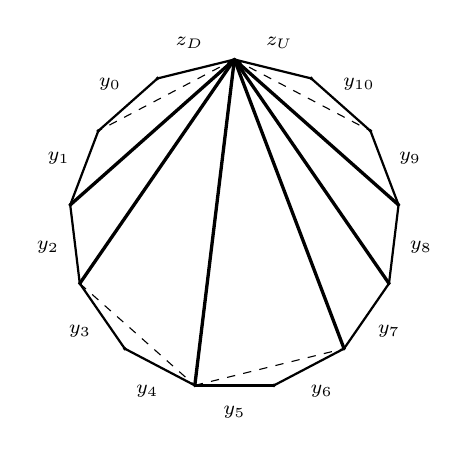
\begin{tikzpicture}[scale=2.1]
\def\n{13}
\foreach \i in {0,...,12} {
  \coordinate (v\i) at ({90+360*(\i)/\n}:1);
}
\foreach \i [evaluate=\i as \j using {int(mod(\i+1,13))}] in {0,...,12} {
  \draw[thick] (v\i) -- (v\j);
}
\foreach \i/\lab in {0/z_D,1/y_0,2/y_1,3/y_2,4/y_3,5/y_4,6/y_5,7/y_6,8/y_7,9/y_8,10/y_9,11/y_{10},12/z_U} {
  \pgfmathtruncatemacro{\j}{mod(\i+1,13)}
  \node[font=\scriptsize] at ($ 1.17*($(v\i)!0.5!(v\j)$) $) {$\lab$};
}
\foreach \k in {3,4,6,8,9,10} { \draw[very thick] (v0) -- (v\k); }
\draw[dashed] (v0) -- (v2);
\draw[dashed] (v0) -- (v11);
\draw[dashed] (v4) -- (v6);
\draw[dashed] (v6) -- (v8);
\foreach \i in {0,...,12} { \fill (v\i) circle (0.012); }
\end{tikzpicture}
\caption{The vertex $\Tstar$. The sides of the $13$-gon carry the thirteen points in their cyclic order,
and a diagonal stands for the cluster of points on the sides it cuts off. Solid: the six fan diagonals
$F_1, F_2, F_4, F_6, F_7, F_8$, $F_k = \{z_D, y_0, \dots, y_k\}$. Dashed: the diagonals of the pairs
$\{z_D, y_0\}$, $\{y_{10}, z_U\}$, $\{y_3, y_4\}$ and $\{y_5, y_6\}$.}
\label{fig:tstar}
\end{figure}

\subsection{The fan chart}
Put $z_D = 0$, $z_U = \infty$ and $y_{10} = 1$, write $q_0 = z_D$ and $q_{k} = y_{k-1}$ for
$k = 1, \dots, 11$, and set $t_k = q_k / q_{k+1} \in (0, 1)$ for $k = 1, \dots, 10$, so that
$q_k = t_k t_{k+1} \cdots t_{10}$. Every bracket factors,
\[
  q_b - q_a = (t_b t_{b+1} \cdots t_{10})\, g(a, b), \qquad g(a, b) = 1 - t_a t_{a+1} \cdots t_{b-1}
  \quad (1 \le a < b),
\]
and $q_b - q_0 = q_b$. Hence the logarithm of every monomial of the tables is
$\sum_k \kappa_k \log t_k + \sum_{a<b} n_{ab} \log g(a,b)$ with integer $\kappa$ and $n$. In this chart
the six fan diagonals of $\Tstar$ are the coordinates $t_2, t_3, t_5, t_7, t_8, t_9$, the pairs
$\{z_D, y_0\}$ and $\{y_{10}, z_U\}$ correspond to $t_1 \to 0$ and $t_{10} \to 0$, and $\{y_3, y_4\}$,
$\{y_5, y_6\}$ to $t_4 \to 1$ and $t_6 \to 1$.

Let $m_1$, $m_2$ be the two monomials of $(C_D)$ in Table~\ref{tab:eqs13}, and let $\Phi$ be the
combination
\[
  \Phi = \log m_{E_1} - \log m_{E_2} + \log m_{E_4} + \log(m_1 + m_2),
\]
where $m_{E_i}$ is the quotient of the two sides of $(E_i)$ in Table~\ref{tab:eqs13}. On $\V$ every term
vanishes, so $\Phi = 0$ on $\V$.

\begin{proposition}\label{prop:phi}
In the fan chart, with $R = m_2/m_1$,
\[
\Phi = \log(1 + R) + \sum_{(a,b) \in N^+} \log g(a,b) - \sum_{(a,b) \in N^-} \log g(a,b),
\]
\begin{align*}
N^+ &= \{(1,8),(2,4),(2,5),(3,7),(4,10),(5,8),(7,9),(8,11),(9,10)\},\\
N^- &= \{(1,4),(2,8),(2,9),(3,5),(4,8),(5,7),(7,10),(8,10),(9,11)\};
\end{align*}
the monomial part cancels. Where $(A_U)$ holds, $R = t_9(1 - t_8)/(1 - t_9)$, so that
$\log(1 + R) = \log g(8,10) - \log g(9,10)$, and
\[
\Phi = t_3 t_4 + t_5 t_6 + t_9 t_{10} + \rho,
\]
where every term of $\rho$ has at least two factors among the fan coordinates
$t_2, t_3, t_5, t_7, t_8, t_9$.
\end{proposition}

\begin{proof}
The first identity is the substitution of the factorisation into the four monomials; the exponents of
$\log t_k$ cancel. Under $(A_U)$ the two terms of $\log(1+R)$ cancel against $(8,10)$ and $(9,10)$, and
$\Phi = \sum \pm \log(1 - \pi_{ab})$ over the remaining eight pairs of each sign, with
$\pi_{ab} = t_a \cdots t_{b-1}$. The three products $\pi_{35} = t_3 t_4$, $\pi_{57} = t_5 t_6$ and
$\pi_{9,11} = t_9 t_{10}$ in $N^-$ contain one fan coordinate each; every other product contains at
least two, and so does every term of order two or more in the expansion of $-\log(1 - \pi)$.
\end{proof}

Near the face on which the six fan coordinates vanish, the equations $(E_2)$--$(E_4)$, $(A_U)$, $(A_D)$
and $(C_D)$ force, at leading order, $t_2 = t_8 = t_9 = t_3$, $t_5 = t_7 = t_3/t_6$ and $t_4 = t_6$; then
$\Phi / t_3 \to t_4 + 1 + t_{10} \ge 1$, and $\Phi = 0$ is impossible. This is the mechanism by which $\V$
avoids the neighbourhood of $\Tstar$ into which the laminar family runs. The certificate of the next
subsection makes it rigorous on explicit regions.

\subsection{The certified neighbourhood}
In the adapted coordinates
\[
\begin{gathered}
e = \log t_3,\quad d = \log(t_6/t_3),\quad \log t_1,\quad \log t_{10},\\
r_2 = \log\frac{t_2}{t_3},\ r_4 = \log\frac{t_4}{t_6},\ r_5 = \log\frac{t_5 t_6}{t_3},\
r_7 = \log\frac{t_7 t_6}{t_3},\ r_8 = \log\frac{t_8}{t_3},\ r_9 = \log\frac{t_9}{t_3},
\end{gathered}
\]
the linear parts of the six monomial equations do not involve the scale $e$, and each of them can be
solved for one coordinate by interval propagation. The quantity $\Phi/t_3$ is evaluated as a signed sum
of terms $\pi\, h(\pi)/t_3$ and $R\,\tilde h(R)/t_3$ with $h(\pi) = -\log(1-\pi)/\pi$ and
$\tilde h(R) = \log(1+R)/R$, which stays accurate as $t_3 \to 0$. A box of the adapted coordinates is
refuted when propagation empties it or when one of the equations, one of the inequalities of $\Lam$, or
$\Phi/t_3$ has a sign on it.

\begin{proposition}\label{prop:RB}
$\V \cap \Lam$ has no point in the region $R = B_1 \cup B_2 \cup B_3 \cup D$ of the fan chart, where
($t_1$ and $t_{10}$ arbitrary throughout)
\begin{align*}
B_1 &= \{t_3 \le 0.1,\ d \ge 2,\ |r_i| \le 2\}, \qquad
B_2 = \{t_3 \le 0.1,\ 0.5 \le d \le 2.2,\ |r_i| \le 0.4\},\\
B_3 &= \{0.1 \le t_3 \le 0.2,\ d \ge 1,\ |r_i| \le 0.25\},\qquad
D = \{t_3 \le 0.1,\ t_k \le 0.95 \text{ for } k = 2, 5, 7, 8, 9\},
\end{align*}
with $i$ ranging over $2, 4, 5, 7, 8, 9$.
\end{proposition}

\begin{proof}[Certificate]
Each of $B_1$, $B_2$, $B_3$ is covered by a branch and bound in the adapted coordinates in which every box
is refuted, in $3{,}567$, $81{,}685$ and $1{,}485{,}235$ boxes. The part of $D$ outside $B_1 \cup B_2$ is
covered by $25$ pieces, $\{d \le 0.5\}$, the twelve pieces $\{0.5 \le d \le 2,\ \pm r_i \ge 0.4\}$ and the
twelve pieces $\{d \ge 2,\ \pm r_i \ge 2\}$, each intersected with $D$, and every piece is closed in the
same way, in $2{,}256{,}565$ boxes in all; in $D$ the bounds
$t_k \le 0.95$ enter the propagation. The arithmetic
is interval arithmetic with outward rounding on logarithms of positive quantities, sums being evaluated as
log-sum-exp and differences only where their sign is known; it is described in
Section~\ref{sec:software}.
\end{proof}

%======================================================================
\section{The certificate}\label{sec:certificate}

\subsection{Boxes}
A \emph{box} is a pair $(T, \beta)$ of a binary tree and a product $\beta = \prod_k I_k$ of closed
intervals $I_k \subset [-\infty, 0]$ in the coordinates $s_k$ of $C_T$, an interval being allowed to be
half-infinite, $I_k = [-\infty, c]$. A box is \emph{closed} when one of the following tests shows that it
contains no point of $\V \cap \Lam$; otherwise it is split.

\begin{enumerate}[label=(\alph*),leftmargin=2em]
\item \emph{Interval test.} By Lemma~\ref{lem:dist} the linear part of each condition is exact and each
correction $x_{ab}$ has an explicit enclosure on the box. If the enclosure of $\log m$ for an equation
$m = 1$ excludes $0$, or that of an inequality lies entirely on the wrong side, the box is closed.

\item \emph{Linear relaxation.} The variables are the ten coordinates $s$, bounded by the box, and the
$66$ corrections $x_{ab}$, bounded by their enclosures. For three points $i < j < k$,
$L_{ik} = L_{ij} + \softplus(L_{jk} - L_{ij})$ with $L = \log \br{\cdot}{\cdot}$ and
$\softplus(u) = \log(1 + e^u)$ convex; this is relaxed by tangent lines of $\softplus$ from below and by its chord over
the enclosure of $L_{jk} - L_{ij}$ from above (by $\softplus(u) \le \softplus(u_1)$ or $\softplus(u) \le u + \softplus(-u_0)$ when
the enclosure is half-infinite). The six monomial equations are linear; the collinearities
$m_1 + m_2 = 1$ and the corner clauses $m_1 + m_2 \le 1$ are relaxed by $m_1, m_2 \le 1$ and by tangent
half-planes of the concave curve $e^{u} + e^{v} = 1$; the non-crossing clauses are linear. All slopes are
dyadic rationals and every constant is computed for its rounded slope and rounded outwards, so each row is
a valid inequality on the whole box. The box is closed when the linear program is infeasible, as shown by
Farkas multipliers $y \ge 0$, $z$ with
\[
  w = A^{\mathsf T} y + E^{\mathsf T} z,\qquad
  \sum_j \min_{v_j \in [\underline v_j, \overline v_j]} w_j v_j \;>\; y^{\mathsf T} b + z^{\mathsf T} c,
\]
the multipliers being computed in floating point \cite{HiGHS} and the inequality checked in exact
rational arithmetic.

\item \emph{Mean-value relaxation.} Each condition is a smooth function of the coordinates. A coordinate
whose interval is half-infinite or wider than $1$ is replaced inside the corrections by
$u_k = e^{s_k} \in [e^{c_0}, e^{c_1}]$ (or $[0, e^{c_1}]$), in which the corrections are smooth up to
$u_k = 0$. With the interval gradient $G$ of the remaining smooth part $h$ over the box, its centre
$z_c$, half-widths $r$ and a dyadic vector $g_0$,
\[
h(z) - g_0 \cdot z \in \bigl[\,h(z_c) - g_0\cdot z_c - R,\ h(z_c) - g_0\cdot z_c + R\,\bigr],\qquad
R = \sum_k \max|G_k - g_{0,k}|\,r_k,
\]
which gives two linear rows for each equation and one for each inequality; trinomials whose two terms
differ on the $u$-coordinates are written as $m_a + \softplus(m_b - m_a)$ with an auxiliary variable for
$m_b - m_a$ and the tangents and chord of $\softplus$. Infeasibility is certified as in (b).

\item \emph{Certified contraction.} When the system of (c) is feasible, each coordinate is minimised and
maximised over it by linear programming, and a slab $\{s_k \le \beta\}$ with $\beta$ below the minimum is
cut off the box if the system together with $s_k \le \beta$ has an exact Farkas certificate; likewise at the
upper end. Every point of $\V \cap \Lam$ in the box lies in the contracted box, with which the branch and
bound continues.

\item \emph{Regions.} The fan coordinates of the box are enclosed, and the box is closed if the enclosure
lies in the region $R$ of Proposition~\ref{prop:RB}.
\end{enumerate}

A box that is not closed is split in one coordinate: after a failed test (c), in the coordinate with the
largest share of the remainders $R$; otherwise in the coordinate whose correction terms are furthest from
their chords. A finite interval is split where the range of $e^{s_k}$ halves, a half-infinite one
$[-\infty, c]$ at $c - \max(2, |c|)$.

\begin{lemma}\label{lem:sound}
If a box is closed by one of the tests (a)--(e), it contains no point of $\V \cap \Lam$.
\end{lemma}

\begin{proof}
For (a) the enclosures contain the values of the conditions at every point of the box. For (b) and (c)
every row is satisfied by every point of $\V \cap \Lam$ in the box, together with the values of the
auxiliary variables at that point, and a Farkas certificate verified exactly shows that no point satisfies
all rows. For (d) the same argument applies to each slab, and the slabs and the contracted box cover the
box. For (e) it is Proposition~\ref{prop:RB}.
\end{proof}

\subsection{The run}
Each of the $58{,}786$ cones is first tested on its root box $(-\infty, 0]^{10}$: $9{,}159$ are closed
there by the interval test, every one of them by the corner clause of $U_4$. The remaining $49{,}627$ are
closed by branch and bound. In each of them the boxes form a binary tree whose leaves are the closed boxes,
$2{,}285{,}836$ in all; Table~\ref{tab:run} summarises the run.

\begin{table}[h]
\centering\small
\begin{tabular}{@{}lr@{}}
\toprule
cones & $58{,}786$ \\
\quad closed at the root & $9{,}159$ \\
\quad closed by branch and bound & $49{,}627$ \\
boxes of the branch and bound & $4{,}522{,}045$ \\
\quad closed by the interval test (a) & $154{,}707$ \\
\quad closed by a linear certificate (b) & $1{,}996{,}263$ \\
\quad closed by the mean-value relaxation (c) & $132{,}058$ \\
\quad closed by the region $D$ (e) & $2{,}808$ \\
\quad split & $2{,}236{,}209$ \\
slabs cut off by certified contraction (d) & $2{,}259{,}157$ \\
largest number of boxes in one cone & $101{,}869$ \\
\bottomrule
\end{tabular}
\caption{The certificate of Theorem~\ref{thm:main}. Of the regions of Proposition~\ref{prop:RB} only $D$
is used, in $16$ cones.}
\label{tab:run}
\end{table}

\begin{proof}[Proof of Theorem~\ref{thm:main}]
The cones cover $\Mo$, the boxes of each cone cover it, and every box is closed. By
Lemma~\ref{lem:sound} no box contains a point of $\V \cap \Lam$.
\end{proof}

\begin{remark}
The theorem was certified a second time by a different decomposition. There, a point at infinity is
fixed and the space is cut into $32{,}805$ cells by the ratios of four gaps between six of the twelve
finite points; the other six are solved for in turn from equations linear in each, and boxes are closed by interval tests, by
linear certificates of the kind in (b) over the $66$ logarithmic distances, and by the regions of
Proposition~\ref{prop:RB}. Six cells, in which the four gap ratios are all extreme, resist this decomposition; they were closed by
the cones of Section~\ref{sec:cones} restricted to the six cells ($32{,}610$ cones, $262{,}314$ boxes,
the region $D$ used for $1{,}959$ of them). Outside these six cells the two certifications share no
decomposition.
\end{remark}

%======================================================================
\part*{II.\quad Circular arcs}
\addcontentsline{toc}{part}{II. Circular arcs}

\section{Circular-arc extended \texorpdfstring{\Sri{}}{Sri} Yantras}\label{sec:arcs}

\subsection{The figure}
We work with generalised circles $\gamma(x,y) = a(x^2+y^2) + bx + cy + d$ as in \cite[\S3]{CK}, so that
lines are the case $a = 0$; the rim is the unit circle, and the axis is $x = 0$. A circular-arc
\Sri{} Yantra is a realisation of the incidence structure of the nine triangles by arcs, symmetric about
the axis \cite[Definition~3.1]{CK}. In \cite{CK} its fourteen outer corners lie on the rim; here they are
released, and the rim is instead met by the extension.

The extension of Section~\ref{sec:figure} takes the following form. The leg of $U_0$ is the generalised
circle through the corners of $D_1$, $D_2$, $D_3$, and the leg of $D_0$ the one through the corners of
$U_1$, $U_2$, $U_3$; their apexes are the poles $(0, 1)$ and $(0, -1)$ of the rim. The base of $U_0$ passes
through the apex of $D_1$, and that of $D_0$ through the apex of $U_1$, as in the straight case. Between
the yantra and the rim the large triangles then form a star, and its points are the cells of a new ring.

\subsection{Walls}\label{sec:walls}
The new ring has two sites, one at each hand of the figure on the downward side and the upward side. On
each site up to three further triangles can be carried out to the rim, namely the three outermost of the
family, read down the page:
\[
\text{down: } D_1,\ D_3,\ D_2, \qquad \text{up: } U_1,\ U_2,\ U_3 .
\]
A triangle is carried out to the rim by extending its legs until they meet a new base. Outermost means
first in the order $D_1, D_3, D_2$ for the downward family, which reads down the page from the top of the
figure, and in the order $U_3, U_2, U_1$ for the upward family, which reads up the page from the bottom.
In each family the outermost carried-out triangle receives the axis-symmetric arc through the tip of the figure, the apex of
$D_1$ for the upward family and that of $U_1$ for the downward, and through the point where its own leg
meets the rim; each further carried-out triangle, going inwards, receives the base given up by the one
outside it; and $U_0$ (or $D_0$) receives the base given up by the innermost. Each carried-out triangle
separates two cells of the ring, and we call it a \emph{wall}. The figure is determined by its two sets of
walls $W_D \subseteq \{D_1, D_3, D_2\}$ and $W_U \subseteq \{U_1, U_2, U_3\}$, and its ring has
\[
  2(|W_D| + 1) + 2(|W_U| + 1) + 2 = 2|W_D| + 2|W_U| + 6
\]
cells, from $6$ to $18$. The outer node of each cell is an apex of $U_0$ or $D_0$ or a corner of a
carried-out triangle, and it is required to lie on the rim.

\begin{definition}\label{def:arcext}
A \emph{circular-arc extended \Sri{} Yantra with walls $(W_D, W_U)$} is a circular-arc \Sri{} Yantra
together with the extension and the carried-out triangles described above, in which the outer nodes of
the new ring lie on the rim and the eleven triangles are laminar.
\end{definition}

We encode a wall pattern by two octal digits $du$, the bits $1, 2, 4$ of $d$ standing for $D_1$, $D_3$,
$D_2$ and those of $u$ for $U_1$, $U_2$, $U_3$. The two figures of Theorem~B have the patterns $22$ and
$36$.

%======================================================================
\section{Constructions}\label{sec:constructions}

\subsection{Moves}
The constructions use the moves of \cite[\S4.2]{CK}, here with the following names: placing a corner
(\texttt{seed}) as a free point, as a height on the axis or as an angle on the rim; pinning a point at a
pole (\texttt{pole}); the axis-symmetric generalised circle through two points (\texttt{s2}, move (B) of
\cite{CK}); the generalised circle through three points (\texttt{s3}, move (C)); and the meeting of two
generalised circles (\texttt{nx}, move (X)), of a generalised circle with the axis (\texttt{na}, move (A))
and with the rim (\texttt{nr}, move (R)). Where a meeting has two points the construction records which,
as in \cite{CK}. An input may be the mirror image of an object already drawn, without that image being a
separate step.

\begin{table}[h]
\centering\small
\begin{tabular}{@{}lrrrrrrrr@{}}
\toprule
& \texttt{seed} & \texttt{pole} & \texttt{s2} & \texttt{s3} & \texttt{nx} & \texttt{na} & \texttt{nr} &
steps \\ \midrule
pattern $22$ & 13 & 2 & 11 & 11 & 21 & 6 & 3 & 67 \\
pattern $36$ & 13 & 2 & 11 & 11 & 23 & 5 & 4 & 69 \\ \bottomrule
\end{tabular}
\caption{The steps of the two constructions. Each draws $22$ curves, the eleven bases and one leg of each
mirror pair of legs, and $45$, respectively $47$, nodes; mirror images complete the figure.}
\label{tab:steps}
\end{table}

\subsection{The two constructions}

\begin{table}[h]
\centering\footnotesize
\begin{tabular}{@{}llrl@{\qquad}llrl@{}}
\toprule
\multicolumn{4}{c}{pattern $22$} & \multicolumn{4}{c}{pattern $36$} \\
\cmidrule(r){1-4}\cmidrule(l){5-8}
corner & placed & & default & corner & placed & & default \\ \midrule
$P_{0}$ & free & 2 & $(0.1943,\ 0.0425)$ & $P_{0}$ & free & 2 & $(0.2863,\ 0.0617)$ \\
$P_{2}$ & free & 2 & $(0.0806,\ -0.0819)$ & $P_{1}$ & free & 2 & $(0.2153,\ -0.0301)$ \\
$P_{7}$ & free & 2 & $(0.0969,\ 0.0473)$ & $P_{3}$ & axis & 1 & $y = -0.2609$ \\
$P_{20}$ & free & 2 & $(0.2664,\ -0.0759)$ & $P_{24}$ & free & 2 & $(0.3989,\ 0.1417)$ \\
$P_{27}$ & axis & 1 & $y = -0.3270$ & $P_{29}$ & free & 2 & $(0.0989,\ 0.1659)$ \\
$P_{29}$ & free & 2 & $(0.0523,\ 0.1215)$ & $P_{34}$ & free & 2 & $(0.3181,\ -0.2469)$ \\
$P_{36}$ & axis & 1 & $y = -0.5095$ & $P_{35}$ & free & 2 & $(0.1596,\ -0.4869)$ \\
$P_{48}$ & free & 2 & $(0.4254,\ -0.1501)$ & $P_{55}$ & axis & 1 & $y = -0.8863$ \\
$P_{53}$ & free & 2 & $(0.0922,\ 0.2053)$ & $P_{61}$ & axis & 1 & $y = 0.5139$ \\
$P_{56}$ & free & 2 & $(0.1640,\ -0.5071)$ & $P_{65}$ & free & 2 & $(0.6663,\ -0.4304)$ \\
$P_{65}$ & free & 2 & $(0.5164,\ -0.3166)$ & $P_{68}$ & axis & 1 & $y = 0.8706$ \\
$P_{68}$ & axis & 1 & $y = 0.7008$ & ring corner 73 & rim & 1 & $\theta = 0.7289$ \\
ring corner 73 & rim & 1 & $\theta = 0.3429$ & ring corner 79 & rim & 1 & $\theta = -0.7334$ \\
\midrule
total & & 22 & & total & & 20 & \\ \bottomrule
\end{tabular}
\caption{The placed corners of the two constructions, the number of real parameters each carries, and its value at the figures of Figure~\ref{fig:two}. Node numbers are those of the accompanying files; the ring corners are numbered from $69$, and a corner on the rim is given by its polar angle.}
\label{tab:seeds}
\end{table}


\begin{proof}[Proof of Theorem~B]
The constructions are those of Tables~\ref{tab:steps22} and \ref{tab:steps36} in
Appendix~\ref{app:constructions}, the sequences \texttt{ARC\_REC2} and \texttt{ARC\_REC3} of the
accompanying viewer; their moves are counted in Table~\ref{tab:steps} and their placed corners listed in
Table~\ref{tab:seeds}. Of the $67$ and $69$ steps, $15$ are placements, $13$ corners and the two poles,
which gives (i).

For (ii), each step draws one node or one curve from objects already drawn and realises the incidences
listed with it: a curve drawn through two or three nodes passes through them, and a node drawn as a
meeting lies on the curves it is the meeting of. Every incidence realised by a step therefore holds
identically wherever the construction is defined, and the outer nodes of the ring lie on the rim because
they are drawn there, either by a meeting with the rim or as the crossing of a leg with a base that was
itself drawn through such a meeting. The steps realise $106$ and $110$ incidences of a node with a side, no
incidence twice. That they are all the incidences of the figure is part of the computation for (iii).

For (iii), the constructions were evaluated in interval arithmetic with outward rounding at sixty
significant digits, from the corners of Table~\ref{tab:seeds} read as exact decimals; a corner on the rim
is the point $(\cos\theta, \sin\theta)$, enclosed by the Taylor series with its remainder. Every meeting
the constructions take exists, its discriminant being enclosed in the positive reals, and the choice between
its two points is decisive; every node is enclosed in a box of width below $10^{-33}$. For every node and
every side not joined by an incidence of the tables, the enclosure of the side's equation at the node
excludes zero, so the figure has no incidence besides those realised by the steps. Each leg is the arc of
its circle from its apex through the nodes on it to its corner. For each pair of a right leg and a right or
left leg of another triangle of the same family, $50$ pairs in each figure (the remaining pairs are their
mirror images), either the two circles do not meet, the enclosure of the discriminant of their meeting
lying below zero, or each of their two meeting points lies strictly on the far side of the chord of one of
the two arcs from the nodes of that arc, and hence off that arc. This was the case for $15$ and $35$ pairs
in pattern $22$ and for $9$ and $41$ pairs in pattern $36$. Hence no leg meets a leg of another triangle of
its family, and the eleven triangles are laminar.
\end{proof}

\begin{remark}
The number of free parameters is the dimension of the family. Evaluating the incidence system of each
figure, every node on every side it is required to lie on and every outer ring node on the rim, at the
default figure, the Jacobian has rank equal to the number of unknowns less $22$, respectively $20$, with a
gap of $10^{-1}$ against $2\times10^{-15}$ in the singular values; the same computation returns $18$ for the
nine-triangle family of \cite{CK}. For pattern $22$ the needs of the objects, counted as in \cite[\S7.1]{CK}, sum to $128 = 22 + 106$, where
$106$ is the number of incidences: an order of the kind used here consumes each incidence exactly once, and
none is arranged; for pattern $36$ they sum to $130 = 20 + 110$.
\end{remark}

%======================================================================
\section{Software and data}\label{sec:software}
\begin{sloppypar}
Everything the proofs use is in the repository of \cite{CK}, \url{https://github.com/michaelkopp/sriyantra}:
the viewer and the GeoGebra files at its top level, and the programs and data of this paper in the folder
\texttt{extended/}.

\paragraph{The viewer and the GeoGebra files.} The viewer \texttt{index.html} draws the two constructed
figures of Theorem~B from their placed corners, in the principal directions of the family or in the
corners themselves, and exports them as SVG or PNG. The files \texttt{sri-yantra-arcs-extended-2.ggb} and
\texttt{sri-yantra-arcs-extended-3.ggb} carry the two constructions as GeoGebra command lists, every step a
\texttt{Circle} through points or an \texttt{Intersect} of two objects, evaluated when the file is opened.
Re-evaluated from their command lists alone by an independent implementation of the operations, they
reproduce all $69$ nodes of the classical figure to $10^{-10}$, every incidence to $1.7\times10^{-15}$ and
$4.4\times10^{-16}$, and the $10$ and $14$ outer nodes of the ring on the rim. Loaded into GeoGebra, they
build $282$ and $300$ commands with nothing undefined, and after each of the $13$ placed corners is dragged
to $60\%$ of its range every incidence still holds to $1.4\times10^{-14}$.

\paragraph{The cone certifier.} In \texttt{extended/certifier/cones/}, \texttt{cone.py} implements the cones, the enclosures of
Lemma~\ref{lem:dist}, the interval test and the linear relaxation with its exact verification;
\texttt{mvf.py} the mean-value relaxation and the certified contraction; \texttt{bbcone.py} the branch
and bound on one cone; \texttt{roots\_all.py} the test of the $58{,}786$ root boxes; \texttt{runcones.py}
and \texttt{run\_all.sh} a resumable parallel run over all cones, and \texttt{summarize.py} the check that
every cone has a closed record. The linear programs are solved by HiGHS \cite{HiGHS} through SciPy; only
their multipliers enter the certificate, and these are verified with Python's exact rationals. Eight test
programs check soundness on samples: boxes, finite, half-infinite and wide, around Newton-polished points
of $\V$ (with the inequalities left out) and of the laminar part of $\V_7$ (with $(E_1)$ left out) must
never be closed, the contracted box must contain the point, and the gradient enclosures of test (c) must
contain the derivatives at random points; each test must print \texttt{PASS}, and \texttt{run\_all.sh}
runs five of them before it starts. The records of Table~\ref{tab:run} amount to $71$ hours of processor time on a
desktop computer with ten cores; the records are in the same folder.

\paragraph{The fan-chart certifier.} In \texttt{extended/certifier/fan/}, \texttt{fanRBB.js} and
\texttt{fanD.js} certify the regions of
Proposition~\ref{prop:RB}, with the arithmetic of \texttt{lg.js}: every quantity is the logarithm of a
positive number, enclosed in an interval with outward padding, sums are evaluated as log-sum-exp, and a
difference is formed only where its sign is known, so that clusters of points at any scale are evaluated
without loss.

\paragraph{The second certification.} The cell decomposition of the remark in
Section~\ref{sec:certificate}, with the records of its runs, is in \texttt{extended/certifier/cells/}.

\paragraph{Exact checks.} In \texttt{extended/check/}, \texttt{straight.py} verifies
Lemma~\ref{lem:widths} in exact rational arithmetic, \texttt{fan.py} the identities of
Proposition~\ref{prop:phi}, and \texttt{gentables.py} produces Tables~\ref{tab:eqs13} and \ref{tab:clauses13} from the data the
certifiers read, so that the tables printed here are the conditions certified.

\paragraph{The constructions of Theorem~B.} \texttt{extended/check/arcs/} holds the two constructions as
read from the viewer (\texttt{recipes.json}), their evaluation in floating point and in interval
arithmetic (\texttt{construct.py}, \texttt{iv.py}), the incidence lists \texttt{incidences\_22.csv} and
\texttt{incidences\_36.csv}, the programs that write Table~\ref{tab:seeds} (\texttt{seedtable.py}) and
Tables~\ref{tab:steps22} and \ref{tab:steps36} (\texttt{steptable.py}), and \texttt{certify.py}, which carries out the computation in the proof of
Theorem~B and writes \texttt{certify.log}. It reproduces the viewer's nodes to $3\times10^{-14}$ at its
default corners.

\paragraph{The figures.} The figures of Part~I are drawn by \texttt{extended/check/drawkites.py} and
\texttt{drawstraight.py} from the points in the same folder, which \texttt{extended/check/fig1/} documents;
those of Part~II are exported from the viewer.

\end{sloppypar}

\section{Concluding remarks}
The straight extension fails, and it fails narrowly. Every condition but one can be met by laminar
figures, and the one that remains, the concurrence of the leg of $D_2$ with the corner of $U_4$, is missed
by an amount that becomes small only where the figure degenerates: near the vertex $\Tstar$, where both
tips press against the apexes of the new triangles. There the miss is of first order in the size of the
degeneration, and the combination $\Phi$ of Proposition~\ref{prop:phi} shows why it cannot vanish.

The method of Part~I applies to any finite system of equations and inequalities between products of
cross-ratios of points on a line. The space of such configurations is not compact, and the conditions
degenerate at its boundary, but the cones of Section~\ref{sec:cones} cover it by finitely many orthants on
each of which every condition is linear up to a correction that is bounded and explicit, and on which a
branch and bound over half-infinite boxes terminates wherever the conditions are separated by a positive
margin in these coordinates. What remains is local: the points of the boundary at which equations and
inequalities meet, here the single vertex $\Tstar$, each of which requires its own analysis.

Four questions remain.
\begin{enumerate}[leftmargin=2em]
\item \emph{A proof without a computer.} Numerically, the residual of $(E_1)$ on the laminar part of
$\V_7$ has infimum zero, approached only at $\Tstar$, so no polynomial certificate of a strict inequality
can exist; a certificate has to vanish at $\Tstar$ to the right order. Is there a short proof of
Theorem~\ref{thm:main} built around Proposition~\ref{prop:phi}?
\item \emph{The other patterns.} Theorem~B gives constructions without arranged coincidences for two of
the $64$ wall patterns. Which of the others are realised by laminar figures, which of those admit such a
construction, and do any require an arranged coincidence in the sense of \cite[\S7.1]{CK}?
\item \emph{Rings on circles.} The ring of cells of an extended figure has its outer nodes on the rim. In
\cite{CK} the grown rings of the nine-triangle figure were asked to have their tips on a circle, which
costs a coincidence that has not been arranged by straightedge and compass. The same question can be
asked of the rings that the extended figures grow outside the rim.
\item \emph{Selection.} As for the nine-triangle figures, the choice of a member of each family is in
the end aesthetic; the members drawn here were chosen by eye.
\end{enumerate}

\appendix
\section{The conditions in the thirteen points}\label{app:tables}
{\small
\begin{longtable}{@{}l>{$}l<{$}@{}}
\caption{The eight equations in the thirteen points, $\br{a}{b} = |p_b - p_a|$, with $a, b$ the levels $0, \dots, 10$ and $D = z_D$, $U = z_U$.}\label{tab:eqs13}\\
\toprule equation & \text{form} \\ \midrule \endfirsthead \toprule equation & \text{form} \\ \midrule \endhead
$E_1$ & \br{1}{4} \br{3}{7} \br{4}{5} \br{6}{8} = \br{1}{3} \br{4}{6} \br{4}{8} \br{5}{7} \\
$E_2$ & \br{0}{3} \br{2}{4} \br{2}{7} \br{6}{9} = \br{0}{2} \br{2}{6} \br{3}{9} \br{4}{7} \\
$E_3$ & \br{0}{3} \br{2}{7} \br{4}{5} \br{7}{9} = \br{0}{2} \br{3}{9} \br{4}{7} \br{5}{7} \\
$E_4$ & \br{1}{3} \br{4}{8} \br{5}{7} \br{7}{10} = \br{1}{7} \br{3}{7} \br{4}{5} \br{8}{10} \\
$A_U$ & \br{0}{7} \br{2}{7} \br{4}{5} \br{9}{U} = \br{0}{2} \br{4}{9} \br{5}{7} \br{7}{U} \\
$A_D$ & \br{D}{1} \br{3}{10} \br{4}{8} \br{5}{7} = \br{D}{3} \br{1}{7} \br{4}{5} \br{8}{10} \\
$C_U$ & 1 = \dfrac{\br{0}{2} \br{1}{7} \br{2}{3} \br{3}{9}}{\br{0}{3} \br{1}{3} \br{2}{7} \br{2}{9}} + \dfrac{\br{0}{2} \br{1}{2} \br{3}{9} \br{3}{10} \br{4}{8} \br{5}{7}}{\br{0}{3} \br{1}{3} \br{2}{7} \br{2}{9} \br{4}{5} \br{8}{10}} \\
$C_D$ & 1 = \dfrac{\br{0}{7} \br{1}{3} \br{2}{7} \br{8}{9}}{\br{0}{2} \br{1}{8} \br{3}{7} \br{7}{9}} + \dfrac{\br{1}{3} \br{4}{9} \br{5}{7} \br{7}{8}}{\br{1}{8} \br{3}{7} \br{4}{5} \br{7}{9}} \\
\bottomrule\end{longtable}

\begin{longtable}{@{}l>{$}l<{$}@{}}
\caption{The twenty-five inequalities that define $\mathcal{L}$. A non-crossing clause $\mathrm{nc}\,AB$ reads $m \ge 1$; a corner clause reads $m_1 + m_2 \le 1$.}\label{tab:clauses13}\\
\toprule clause & \text{form} \\ \midrule \endfirsthead \toprule clause & \text{form} \\ \midrule \endhead
non-crossing $D_1D_2$ & \br{0}{7} \br{1}{3} \br{2}{7} \ge \br{0}{2} \br{1}{7} \br{3}{7} \\
non-crossing $D_1D_3$ & \br{0}{7} \br{2}{7} \br{4}{5} \ge \br{0}{2} \br{4}{7} \br{5}{7} \\
non-crossing $D_1D_4$ & \br{0}{6} \br{2}{4} \br{2}{7} \ge \br{0}{2} \br{2}{6} \br{4}{7} \\
non-crossing $D_1D_5$ & \br{0}{5} \br{2}{7} \br{4}{5} \br{6}{8} \ge \br{0}{2} \br{4}{6} \br{5}{7} \br{5}{8} \\
non-crossing $D_2D_3$ & \br{1}{8} \br{3}{7} \br{4}{5} \ge \br{1}{3} \br{4}{8} \br{5}{7} \\
non-crossing $D_2D_4$ & \br{1}{6} \br{2}{4} \br{3}{7} \ge \br{1}{3} \br{2}{6} \br{4}{7} \\
non-crossing $D_2D_5$ & \br{1}{5} \br{3}{7} \br{4}{5} \br{6}{8} \ge \br{1}{3} \br{4}{6} \br{5}{7} \br{5}{8} \\
non-crossing $D_4D_3$ & \br{2}{6} \br{4}{5} \br{4}{7} \ge \br{2}{4} \br{4}{6} \br{5}{7} \\
non-crossing $D_4D_5$ & \br{2}{5} \br{4}{5} \br{4}{7} \br{6}{8} \ge \br{2}{4} \br{4}{6} \br{5}{7} \br{5}{8} \\
non-crossing $D_5D_3$ & \br{4}{6} \br{5}{8} \ge \br{4}{5} \br{6}{8} \\
non-crossing $U_1U_2$ & \br{0}{2} \br{3}{10} \br{4}{8} \br{5}{7} \ge \br{0}{3} \br{2}{7} \br{4}{5} \br{8}{10} \\
non-crossing $U_1U_3$ & \br{3}{10} \br{4}{8} \br{5}{7} \ge \br{3}{7} \br{4}{5} \br{8}{10} \\
non-crossing $U_1U_4$ & \br{4}{10} \br{6}{8} \ge \br{4}{6} \br{8}{10} \\
non-crossing $U_2U_3$ & \br{0}{3} \br{2}{9} \ge \br{0}{2} \br{3}{9} \\
non-crossing $U_2U_4$ & \br{0}{3} \br{2}{7} \br{4}{5} \br{4}{9} \br{6}{8} \ge \br{0}{2} \br{3}{9} \br{4}{6} \br{4}{8} \br{5}{7} \\
non-crossing $U_4U_3$ & \br{4}{6} \br{4}{8} \br{5}{7} \ge \br{4}{5} \br{4}{7} \br{6}{8} \\
corner $U_1$ & \dfrac{\br{0}{2} \br{3}{10} \br{4}{8} \br{5}{7} \br{7}{9}}{\br{0}{7} \br{2}{7} \br{3}{9} \br{4}{5} \br{8}{10}} + \dfrac{\br{0}{2} \br{3}{7} \br{4}{9} \br{5}{7}}{\br{0}{7} \br{2}{7} \br{3}{9} \br{4}{5}} \le 1 \\
corner $U_2$ & \dfrac{\br{0}{3} \br{7}{9}}{\br{0}{7} \br{3}{9}} + \dfrac{\br{0}{2} \br{4}{9} \br{5}{7}}{\br{0}{7} \br{2}{9} \br{4}{5}} \le 1 \\
corner $U_3$ & \dfrac{\br{0}{2} \br{1}{7} \br{7}{9}}{\br{0}{7} \br{1}{9} \br{2}{7}} + \dfrac{\br{0}{2} \br{1}{7} \br{4}{9} \br{5}{7}}{\br{0}{7} \br{1}{9} \br{2}{7} \br{4}{5}} \le 1 \\
corner $U_4$ & \dfrac{\br{0}{2} \br{4}{6} \br{4}{8} \br{5}{7} \br{7}{9}}{\br{0}{7} \br{2}{7} \br{4}{5} \br{4}{9} \br{6}{8}} + \dfrac{\br{0}{2} \br{4}{7} \br{5}{7}}{\br{0}{7} \br{2}{7} \br{4}{5}} \le 1 \\
corner $D_1$ & \dfrac{\br{0}{7} \br{1}{3} \br{2}{7} \br{4}{5} \br{8}{10}}{\br{0}{2} \br{1}{7} \br{3}{10} \br{4}{8} \br{5}{7}} + \dfrac{\br{3}{7} \br{4}{5} \br{8}{10}}{\br{3}{10} \br{4}{8} \br{5}{7}} \le 1 \\
corner $D_2$ & \dfrac{\br{3}{7} \br{4}{5} \br{8}{10}}{\br{3}{10} \br{4}{8} \br{5}{7}} + \dfrac{\br{1}{7} \br{3}{8} \br{4}{5} \br{8}{10}}{\br{1}{8} \br{3}{10} \br{4}{8} \br{5}{7}} \le 1 \\
corner $D_3$ & \dfrac{\br{1}{3} \br{4}{9} \br{8}{10}}{\br{1}{9} \br{3}{10} \br{4}{8}} + \dfrac{\br{1}{7} \br{3}{9} \br{4}{5} \br{8}{10}}{\br{1}{9} \br{3}{10} \br{4}{8} \br{5}{7}} \le 1 \\
corner $D_4$ & \dfrac{\br{1}{3} \br{2}{6} \br{4}{5} \br{4}{7} \br{8}{10}}{\br{1}{6} \br{2}{4} \br{3}{10} \br{4}{8} \br{5}{7}} + \dfrac{\br{1}{7} \br{3}{6} \br{4}{5} \br{8}{10}}{\br{1}{6} \br{3}{10} \br{4}{8} \br{5}{7}} \le 1 \\
corner $D_5$ & \dfrac{\br{1}{3} \br{4}{6} \br{5}{8} \br{8}{10}}{\br{1}{5} \br{3}{10} \br{4}{8} \br{6}{8}} + \dfrac{\br{1}{7} \br{3}{5} \br{4}{5} \br{8}{10}}{\br{1}{5} \br{3}{10} \br{4}{8} \br{5}{7}} \le 1 \\
\bottomrule\end{longtable}
}

\section{The two constructions}\label{app:constructions}
Tables~\ref{tab:steps22} and \ref{tab:steps36} list the steps of the constructions of Theorem~B in the
order in which they are taken. Each row gives the object drawn and the objects it is drawn from; the
incidences a step realises are those between the object drawn and the objects listed with it.

\begin{table}[p]
\centering\scriptsize
\setlength{\tabcolsep}{3.2pt}
\begin{tabular}{@{}rlll@{\qquad}rlll@{}}
\toprule
& drawn & from & position & & drawn & from & position \\ \midrule
1 & $P_{69}$ & pole & $(0.000, -1.000)$ & 35 & $\beta(D_{0})$ & $P_{61}, P_{73}$ &  \\
2 & $P_{70}$ & pole & $(0.000, 1.000)$ & 36 & $P_{31}$ & $\beta(D_{0}) \cap \lambda(U_{0})$ & $(0.511, 0.344)$ \\
3 & $P_{65}$ & placed & $(0.516, -0.317)$ & 37 & $\lambda(D_{3})$ & $P_{20}, P_{31}, P_{36}$ &  \\
4 & $P_{73}$ & placed on the rim & $(0.942, 0.336)$ & 38 & $P_{71}$ & $\lambda(D_{3}) \cap \text{rim}$ & $(0.711, 0.703)$ \\
5 & $\lambda(D_{0})$ & $P_{65}, P_{69}, P_{73}$ &  & 39 & $\beta(D_{3})$ & $P_{68}, P_{71}$ &  \\
6 & $P_{56}$ & placed & $(0.164, -0.507)$ & 40 & $P_{35}$ & $\beta(U_{0}) \cap \lambda(D_{3})$ & $(0.114, -0.326)$ \\
7 & $P_{29}$ & placed & $(0.052, 0.121)$ & 41 & $P_{34}$ & $\lambda(D_{3}) \cap \lambda(U_{3})$ & $(0.215, -0.161)$ \\
8 & $P_{20}$ & placed & $(0.266, -0.076)$ & 42 & $P_{32}$ & $\beta(D_{2}) \cap \lambda(D_{3})$ & $(0.423, 0.191)$ \\
9 & $P_{48}$ & placed & $(0.425, -0.150)$ & 43 & $\beta(U_{1})$ & $P_{34}, P_{48}$ &  \\
10 & $P_{53}$ & placed & $(0.092, 0.205)$ & 44 & $P_{47}$ & $\beta(U_{1}) \cap \lambda(D_{0})$ & $(0.643, -0.132)$ \\
11 & $P_{2}$ & placed & $(0.081, -0.082)$ & 45 & $P_{3}$ & $\beta(U_{1}) \cap \text{axis}$ & $(0.000, -0.164)$ \\
12 & $\beta(U_{4})$ & $P_{2}, P_{20}$ &  & 46 & $\lambda(U_{1})$ & $P_{32}, P_{47}, P_{68}$ &  \\
13 & $P_{16}$ & $\beta(U_{4}) \cap \text{axis}$ & $(0.000, -0.083)$ & 47 & $\lambda(D_{5})$ & $P_{0}, P_{2}, P_{3}$ &  \\
14 & $P_{36}$ & placed on the axis & $(0.000, -0.509)$ & 48 & $P_{13}$ & $\beta(D_{0}) \cap \lambda(U_{1})$ & $(0.305, 0.347)$ \\
15 & $\beta(U_{3})$ & $P_{36}, P_{56}$ &  & 49 & $P_{1}$ & $\lambda(D_{5}) \cap \lambda(U_{3})$ & $(0.137, -0.021)$ \\
16 & $P_{44}$ & $\beta(U_{3}) \cap \lambda(D_{0})$ & $(0.388, -0.496)$ & 50 & $P_{57}$ & $\lambda(D_{2}) \cap \lambda(U_{1})$ & $(0.542, 0.023)$ \\
17 & $P_{27}$ & placed on the axis & $(0.000, -0.327)$ & 51 & $\lambda(D_{1})$ & $P_{7}, P_{13}, P_{16}$ &  \\
18 & $\beta(U_{0})$ & $P_{27}, P_{65}$ &  & 52 & $P_{9}$ & $\lambda(D_{1}) \cap \lambda(U_{0})$ & $(0.400, 0.493)$ \\
19 & $P_{75}$ & $\beta(U_{0}) \cap \text{rim}$ & $(0.957, -0.291)$ & 53 & $P_{15}$ & $\lambda(D_{1}) \cap \lambda(U_{4})$ & $(0.148, 0.118)$ \\
20 & $P_{7}$ & placed & $(0.097, 0.047)$ & 54 & $\beta(D_{4})$ & $P_{15}, P_{29}$ &  \\
21 & $\lambda(U_{3})$ & $P_{7}, P_{29}, P_{44}$ &  & 55 & $P_{14}$ & $\beta(D_{2}) \cap \lambda(D_{1})$ & $(0.207, 0.202)$ \\
22 & $P_{46}$ & $\lambda(U_{3}) \cap \text{axis}$ & $(0.000, 0.206)$ & 56 & $\lambda(U_{2})$ & $P_{14}, P_{48}, P_{65}$ &  \\
23 & $\beta(D_{2})$ & $P_{46}, P_{53}$ &  & 57 & $P_{67}$ & $\lambda(U_{2}) \cap \text{axis}$ & $(0.000, 0.491)$ \\
24 & $P_{21}$ & $\beta(U_{4}) \cap \lambda(U_{3})$ & $(0.171, -0.080)$ & 58 & $P_{33}$ & $\lambda(D_{3}) \cap \lambda(U_{2})$ & $(0.324, 0.021)$ \\
25 & $P_{45}$ & $\beta(U_{0}) \cap \lambda(U_{3})$ & $(0.302, -0.323)$ & 59 & $P_{38}$ & $\beta(D_{0}) \cap \lambda(U_{2})$ & $(0.107, 0.348)$ \\
26 & $\lambda(D_{2})$ & $P_{45}, P_{48}, P_{56}$ &  & 60 & $\beta(D_{1})$ & $P_{9}, P_{67}$ &  \\
27 & $P_{55}$ & $\lambda(D_{2}) \cap \text{axis}$ & $(0.000, -0.712)$ & 61 & $P_{10}$ & $\beta(D_{1}) \cap \lambda(U_{1})$ & $(0.186, 0.492)$ \\
28 & $P_{52}$ & $\beta(D_{2}) \cap \lambda(D_{2})$ & $(0.637, 0.172)$ & 62 & $P_{77}$ & $\lambda(U_{2}) \cap \text{rim}$ & $(0.704, -0.710)$ \\
29 & $\lambda(U_{0})$ & $P_{52}, P_{70}, P_{75}$ &  & 63 & $\beta(U_{2})$ & $P_{55}, P_{77}$ &  \\
30 & $P_{68}$ & placed on the axis & $(0.000, 0.701)$ & 64 & $P_{24}$ & $\beta(D_{4}) \cap \lambda(U_{2})$ & $(0.270, 0.107)$ \\
31 & $P_{0}$ & placed & $(0.194, 0.043)$ & 65 & $\lambda(D_{4})$ & $P_{21}, P_{24}, P_{27}$ &  \\
32 & $\beta(D_{5})$ & $P_{0}, P_{7}$ &  & 66 & $P_{26}$ & $\beta(U_{1}) \cap \lambda(D_{4})$ & $(0.118, -0.163)$ \\
33 & $\lambda(U_{4})$ & $P_{0}, P_{20}, P_{53}$ &  & 67 & $P_{25}$ & $\lambda(D_{4}) \cap \lambda(U_{4})$ & $(0.218, 0.004)$ \\
34 & $P_{61}$ & $\lambda(U_{4}) \cap \text{axis}$ & $(0.000, 0.348)$ &  &  &  &  \\
\bottomrule
\end{tabular}
\caption{The construction of pattern $22$, step by step. $\beta(T)$ is the base of $T$, $\lambda(T)$ its right leg and $\lambda^\prime(T)$ its left leg, and $P^\prime$ is the mirror image of $P$. A curve is drawn through the nodes listed, and a node as the meeting listed; of the two points of a meeting it is the one at the position given, which is its position at the corners of Table~\ref{tab:seeds} to three decimals.}
\label{tab:steps22}
\end{table}

\begin{table}[p]
\centering\scriptsize
\setlength{\tabcolsep}{3.2pt}
\begin{tabular}{@{}rlll@{\qquad}rlll@{}}
\toprule
& drawn & from & position & & drawn & from & position \\ \midrule
1 & $P_{69}$ & pole & $(0.000, -1.000)$ & 36 & $P_{67}$ & $\lambda(U_{2}) \cap \text{axis}$ & $(0.000, 0.693)$ \\
2 & $P_{70}$ & pole & $(0.000, 1.000)$ & 37 & $\beta(D_{3})$ & $P_{67}, P_{73}$ &  \\
3 & $P_{73}$ & placed on the rim & $(0.746, 0.666)$ & 38 & $\lambda(D_{0})$ & $P_{44}, P_{65}, P_{69}$ &  \\
4 & $P_{68}$ & placed on the axis & $(0.000, 0.871)$ & 39 & $P_{47}$ & $\beta(U_{1}) \cap \lambda(D_{0})$ & $(0.803, -0.171)$ \\
5 & $P_{61}$ & placed on the axis & $(0.000, 0.514)$ & 40 & $P_{75}$ & $\lambda(D_{0}) \cap \text{rim}$ & $(0.920, 0.392)$ \\
6 & $P_{35}$ & placed & $(0.160, -0.487)$ & 41 & $\beta(D_{0})$ & $P_{61}, P_{75}$ &  \\
7 & $P_{24}$ & placed & $(0.399, 0.142)$ & 42 & $P_{31}$ & $\beta(D_{0}) \cap \lambda(D_{3})$ & $(0.667, 0.450)$ \\
8 & $P_{3}$ & placed on the axis & $(0.000, -0.261)$ & 43 & $P_{38}$ & $\beta(D_{0}) \cap \lambda(U_{2})$ & $(0.151, 0.511)$ \\
9 & $P_{0}$ & placed & $(0.286, 0.062)$ & 44 & $\lambda(U_{0})$ & $P_{31}, P_{70}, P_{77}$ &  \\
10 & $P_{29}$ & placed & $(0.099, 0.166)$ & 45 & $P_{9}$ & $\beta(D_{3}) \cap \lambda(U_{0})$ & $(0.474, 0.682)$ \\
11 & $\beta(D_{4})$ & $P_{24}, P_{29}$ &  & 46 & $P_{52}$ & $\lambda(D_{2}) \cap \lambda(U_{0})$ & $(0.803, 0.202)$ \\
12 & $P_{34}$ & placed & $(0.318, -0.247)$ & 47 & $\beta(D_{2})$ & $P_{46}, P_{52}$ &  \\
13 & $\lambda(D_{3})$ & $P_{34}, P_{35}, P_{73}$ &  & 48 & $P_{14}$ & $\beta(D_{2}) \cap \lambda(U_{2})$ & $(0.307, 0.291)$ \\
14 & $\beta(U_{1})$ & $P_{3}, P_{34}$ &  & 49 & $P_{32}$ & $\beta(D_{2}) \cap \lambda(D_{3})$ & $(0.583, 0.252)$ \\
15 & $P_{36}$ & $\lambda(D_{3}) \cap \text{axis}$ & $(0.000, -0.699)$ & 50 & $\lambda(U_{1})$ & $P_{32}, P_{47}, P_{68}$ &  \\
16 & $P_{1}$ & placed & $(0.215, -0.030)$ & 51 & $P_{57}$ & $\lambda(D_{2}) \cap \lambda(U_{1})$ & $(0.716, 0.021)$ \\
17 & $\lambda(U_{3})$ & $P_{1}, P_{29}, P_{34}$ &  & 52 & $P_{10}$ & $\beta(D_{3}) \cap \lambda(U_{1})$ & $(0.215, 0.691)$ \\
18 & $\lambda(D_{5})$ & $P_{0}, P_{1}, P_{3}$ &  & 53 & $P_{13}$ & $\beta(D_{0}) \cap \lambda(U_{1})$ & $(0.405, 0.491)$ \\
19 & $P_{81}$ & $\lambda(U_{3}) \cap \text{rim}$ & $(0.488, -0.873)$ & 54 & $\lambda(D_{1})$ & $P_{9}, P_{13}, P_{14}$ &  \\
20 & $P_{46}$ & $\lambda(U_{3}) \cap \text{axis}$ & $(0.000, 0.306)$ & 55 & $P_{7}$ & $\lambda(D_{1}) \cap \lambda(U_{3})$ & $(0.160, 0.067)$ \\
21 & $P_{65}$ & placed & $(0.666, -0.430)$ & 56 & $P_{15}$ & $\beta(D_{4}) \cap \lambda(D_{1})$ & $(0.226, 0.159)$ \\
22 & $\beta(U_{0})$ & $P_{35}, P_{65}$ &  & 57 & $P_{71}$ & $\lambda(D_{1}) \cap \text{rim}$ & $(0.519, 0.855)$ \\
23 & $P_{45}$ & $\beta(U_{0}) \cap \lambda(U_{3})$ & $(0.399, -0.469)$ & 58 & $\beta(D_{1})$ & $P_{68}, P_{71}$ &  \\
24 & $P_{77}$ & $\beta(U_{0}) \cap \text{rim}$ & $(0.928, -0.373)$ & 59 & $\beta(D_{5})$ & $P_{0}, P_{7}$ &  \\
25 & $P_{27}$ & $\beta(U_{0}) \cap \text{axis}$ & $(0.000, -0.490)$ & 60 & $P_{16}$ & $\lambda(D_{1}) \cap \text{axis}$ & $(0.000, -0.120)$ \\
26 & $P_{55}$ & placed on the axis & $(0.000, -0.886)$ & 61 & $\lambda(U_{4})$ & $P_{0}, P_{15}, P_{61}$ &  \\
27 & $\beta(U_{3})$ & $P_{55}, P_{81}$ &  & 62 & $P_{53}$ & $\beta(D_{2}) \cap \lambda(U_{4})$ & $(0.135, 0.303)$ \\
28 & $P_{79}$ & placed on the rim & $(0.743, -0.669)$ & 63 & $P_{20}$ & $\lambda(D_{3}) \cap \lambda(U_{4})$ & $(0.395, -0.117)$ \\
29 & $\lambda(U_{2})$ & $P_{24}, P_{65}, P_{79}$ &  & 64 & $\beta(U_{4})$ & $P_{16}, P_{20}$ &  \\
30 & $\beta(U_{2})$ & $P_{36}, P_{79}$ &  & 65 & $P_{2}$ & $\beta(U_{4}) \cap \lambda(D_{5})$ & $(0.139, -0.119)$ \\
31 & $P_{33}$ & $\lambda(D_{3}) \cap \lambda(U_{2})$ & $(0.468, 0.017)$ & 66 & $P_{21}$ & $\beta(U_{4}) \cap \lambda(U_{3})$ & $(0.260, -0.118)$ \\
32 & $P_{48}$ & $\beta(U_{1}) \cap \lambda(U_{2})$ & $(0.580, -0.214)$ & 67 & $\lambda(D_{4})$ & $P_{21}, P_{24}, P_{27}$ &  \\
33 & $P_{44}$ & $\beta(U_{2}) \cap \lambda(U_{3})$ & $(0.456, -0.688)$ & 68 & $P_{26}$ & $\beta(U_{1}) \cap \lambda(D_{4})$ & $(0.173, -0.257)$ \\
34 & $\lambda(D_{2})$ & $P_{45}, P_{48}, P_{55}$ &  & 69 & $P_{25}$ & $\lambda(D_{4}) \cap \lambda(U_{4})$ & $(0.326, -0.003)$ \\
35 & $P_{56}$ & $\beta(U_{2}) \cap \lambda(D_{2})$ & $(0.200, -0.697)$ &  &  &  &  \\
\bottomrule
\end{tabular}
\caption{The construction of pattern $36$, step by step. $\beta(T)$ is the base of $T$, $\lambda(T)$ its right leg and $\lambda^\prime(T)$ its left leg, and $P^\prime$ is the mirror image of $P$. A curve is drawn through the nodes listed, and a node as the meeting listed; of the two points of a meeting it is the one at the position given, which is its position at the corners of Table~\ref{tab:seeds} to three decimals.}
\label{tab:steps36}
\end{table}

\clearpage

\begin{thebibliography}{99}
\bibitem{Brown} F.~Brown, Multiple zeta values and periods of moduli spaces
$\overline{\mathfrak{M}}_{0,n}$, \emph{Ann. Sci. \'Ec. Norm. Sup\'er.} (4) \textbf{42} (2009), no.~3,
371--489.
\bibitem{Chiodo} A.~Chiodo, On the construction of the \Sri{} Yantra, \emph{C. R. Math. Acad. Sci. Paris}
\textbf{359} (2021), no.~4, 377--397. doi:10.5802/crmath.163
\bibitem{CK} Claude and M.~Kopp, \emph{The circular-arc \Sri{} Yantra}, 2026.
\url{https://github.com/michaelkopp/sriyantra}
\bibitem{HiGHS} Q.~Huangfu and J.~A.~J.~Hall, Parallelizing the dual revised simplex method,
\emph{Math. Program. Comput.} \textbf{10} (2018), 119--142.
\bibitem{Vuillemin} J.~Vuillemin, A unifying look at data structures, \emph{Comm. ACM} \textbf{23} (1980),
no.~4, 229--239.
\end{thebibliography}

\end{document}
